\documentclass[a4paper,10pt
,draft
%, final
]{article}%





% ---- Commands on draft --------

\usepackage[dvipsnames]{xcolor}% adds colors
\usepackage{ifdraft}[pos=0.8]
\ifdraft{
  \color[RGB]{63,63,63}
%  \pagecolor[RGB]{220,220,204}
  \usepackage[notref]{showkeys} % notref - don't show reference names, only labels
  \usepackage{todonotes}
}
{
  \usepackage[disable]{todonotes}
}

\pdfcompresslevel=0
\pdfobjcompresslevel=0


\usepackage{xr-hyper} % for \externaldocument
\externaldocument[OC-]{OneColor} % cite using names from other half
\externaldocument[AC-]{AllColors} % cite using names from other half
\externaldocument[TAS-]{TameAndSquare} % cite using names from other half


\usepackage[pagebackref, colorlinks, citecolor=PineGreen, linkcolor=PineGreen]{hyperref}
\hypersetup{
  final,
  pdftitle={Rigidification of dendroidal $\infty$-operads}
  pdfauthor={Bonventre, P. and Pereira, L. A.},
  linktoc=page,
  pdfpagemode=UseNone,
  pdfpagelayout=SinglePage,
}






\usepackage{amsmath, amsthm}% {amsfonts, amssymb}

% ------ New Characters --------------------------------------

\let\llhook\lhook
\usepackage[latin1]{inputenc}%
%\usepackage[T1]{fontenc}
\usepackage{MnSymbol}
\usepackage[
cal = cm,
bb = ams,
frak = euler,
scr = rsfs
]{mathalpha}

% \DeclareMathAlphabet\mathbb{U}{msb}{m}{n}
% %\usepackage{stmaryrd}
% %\usepackage{upgreek}
% \usepackage{mathrsfs}
% % \usepackage[english]{babel}
% % \usepackage{fouriernc}
% % \DeclareMathAlphabet{\mathscr}{U}{mathrsfs}{m}{n}`
% %\usepackage{pifont}
% %\newcommand{\cmark}{\text{\ding{51}}}
% %\newcommand{\xmark}{\text{\ding{55}}}

\usepackage[normalem]{ulem} % underlining
% \usepackage{dsfont} % double strike-through
% \usepackage{bbm} % more blackboard bold



%----- Enumerate ---------------------------------------------
% \usepackage{paralist} % for inparaenum
% \usepackage{enumerate}%
\usepackage[inline,shortlabels]{enumitem}%
\setenumerate{label=(\roman*)}

% ---------- Page Typesetting ----------
\usepackage[final]{microtype}
\usepackage{relsize}
\usepackage{geometry}

%-------- Tikz ---------------------------

\usepackage{tikz}%
\usetikzlibrary{matrix,arrows,decorations.pathmorphing,
cd,patterns,calc}
\tikzset{%
  % treenode/.style = {shape=rectangle, rounded corners, draw, align=center, font=\footnotesize,
  %                    top color=white, bottom color=blue!20},%
  % root/.style     = {treenode, font=\Large, bottom color=red!30},%
  % env/.style      = {treenode, font=\ttfamily\normalsize},%
  dummy/.style    = {circle,draw,inner sep=0pt,minimum size=2mm}%
}%

\usetikzlibrary[decorations.pathreplacing]




% ----- Labels Changed? --------

\makeatletter

\def\@testdef #1#2#3{%
  \def\reserved@a{#3}\expandafter \ifx \csname #1@#2\endcsname
  \reserved@a  \else
  \typeout{^^Jlabel #2 changed:^^J%
    \meaning\reserved@a^^J%
    \expandafter\meaning\csname #1@#2\endcsname^^J}%
  \@tempswatrue \fi}

\makeatother

%%%%%%%%%%%%%%%%%%%%%%%%% INTERNAL REFERENCES %%%%%%%%%%%%%%%%%%%%%%%%%%%%%%%%%%%

\numberwithin{equation}{section} 
\numberwithin{figure}{section}

\usepackage{mathtools}
\mathtoolsset{showonlyrefs,showmanualtags} % Only number equations which are referenced with eqref


% ------- New Theorems/ Definition/ Names-----------------------

 % \theoremstyle{plain} % bold name, italic text
\newtheorem{theorem}[equation]{Theorem}%
\newtheorem*{theorem*}{Theorem}%
\newtheorem{lemma}[equation]{Lemma}%
\newtheorem{proposition}[equation]{Proposition}%
\newtheorem{corollary}[equation]{Corollary}%
\newtheorem{conjecture}[equation]{Conjecture}%
\newtheorem*{conjecture*}{Conjecture}%
\newtheorem{claim}[equation]{Claim}%

%%%%%% Fancy Numbering for Theorems
\newtheorem{innercustomgeneric}{\customgenericname}
\providecommand{\customgenericname}{}
\newcommand{\newcustomtheorem}[2]{%
  \newenvironment{#1}[1]
  {%
   \renewcommand\customgenericname{#2}%
   \renewcommand\theinnercustomgeneric{##1}%
   \innercustomgeneric
  }
  {\endinnercustomgeneric}
}

\newcustomtheorem{customthm}{Theorem}
\newcustomtheorem{customprop}{Proposition}
\newcustomtheorem{customcor}{Corollary}
%%%%%%%%%%%%%

\theoremstyle{definition} % bold name, plain text
\newtheorem{definition}[equation]{Definition}%
\newtheorem*{definition*}{Definition}%
\newtheorem{example}[equation]{Example}%
\newtheorem{remark}[equation]{Remark}%
\newtheorem{notation}[equation]{Notation}%
\newtheorem{convention}[equation]{Convention}%
\newtheorem{assumption}[equation]{Assumption}%
\newtheorem{exercise}{Exercise}%


% %%%%%%%%%%%%%%%%%%%%%%%%%%%%%%%%%%%%%%%%%%%%%%%%%%%%%%%%%%%%%%%%%%%%%%%%%%%%%%%%
% ------------------------------ COMMANDS ------------------------------

% ---------- macros

\newcommand{\set}[1]{\left\{#1\right\}}%
\newcommand{\sets}[2]{\left\{ #1 \;|\; #2\right\}}%
\newcommand{\longto}{\longrightarrow}%
\newcommand{\into}{\hookrightarrow}%
\newcommand{\onto}{\twoheadrightarrow}%

\usepackage{harpoon}
\newcommand{\vect}[1]{\text{\overrightharp{\ensuremath{#1}}}}


% ---------- operators

\newcommand{\Sym}{\ensuremath{\mathsf{Sym}}}%
\newcommand{\Fin}{\mathsf{F}}%
\newcommand{\Set}{\ensuremath{\mathsf{Set}}}
\newcommand{\Top}{\ensuremath{\mathsf{Top}}}
\newcommand{\sSet}{\ensuremath{\mathsf{sSet}}}%
\newcommand{\Cat}{\mathsf{Cat}}
\newcommand{\sCat}{\mathsf{sCat}}
\newcommand{\Op}{\mathsf{Op}}%
\newcommand{\sOp}{\ensuremath{\mathsf{sOp}}}%
\newcommand{\sSym}{\ensuremath{\mathsf{sSym}}}%
\newcommand{\fgt}{\ensuremath{\mathsf{fgt}}}%
\newcommand{\dSet}{\mathsf{dSet}}
\newcommand{\sdSet}{\mathsf{sdSet}}
\newcommand{\PreOp}{\mathsf{PreOp}}
\newcommand{\Fun}{\mathsf{Fun}}
\newcommand{\Fib}{\mathsf{Fib}}
\newcommand{\Alg}{\mathsf{Alg}}
\newcommand{\Kl}{\mathsf{Kl}}



\DeclareMathOperator{\hocmp}{hocmp}%
\DeclareMathOperator{\cmp}{cmp}%
\DeclareMathOperator{\hofiber}{hofiber}%
\DeclareMathOperator{\fiber}{fiber}%
\DeclareMathOperator{\hocofiber}{hocof}%
\DeclareMathOperator{\hocof}{hocof}%
\DeclareMathOperator{\holim}{holim}%
\DeclareMathOperator{\hocolim}{hocolim}%
\DeclareMathOperator{\colim}{colim}%
\DeclareMathOperator{\Lan}{Lan}%
\DeclareMathOperator{\Ran}{Ran}%
\DeclareMathOperator{\Map}{Map}%
\DeclareMathOperator{\Id}{Id}%
\DeclareMathOperator{\mlf}{mlf}%
\DeclareMathOperator{\Hom}{Hom}%
\DeclareMathOperator{\Ho}{Ho}
\DeclareMathOperator{\Aut}{Aut}%
\DeclareMathOperator{\Stab}{Stab}
\DeclareMathOperator{\Iso}{Iso}
\DeclareMathOperator{\Ob}{Ob}

% ---------- shortcuts

\newcommand{\F}{\ensuremath{\mathcal F}}
\newcommand{\V}{\ensuremath{\mathcal V}}
\newcommand{\Q}{\ensuremath{\mathcal Q}}
\renewcommand{\O}{\ensuremath{\mathcal O}}
\renewcommand{\P}{\ensuremath{\mathcal P}}
\newcommand{\C}{\ensuremath{\mathcal C}}
\newcommand{\A}{\ensuremath{\mathcal A}}

\newcommand{\del}{\partial}%

\newcommand{\ki}{\chi}
\newcommand{\ksi}{\xi}
\newcommand{\Ksi}{\Xi}

\newcommand{\lltimes}{\underline{\ltimes}}

% detecting $\V$-categories:

\newcommand{\I}{\mathbb I}
\newcommand{\J}{\mathbb J}
\newcommand{\1}{\ensuremath{\mathbbm 1}}%{\ensuremath{\mathbb{id}}} %\eta

% lazy shortcuts

\newcommand{\SC}{\Sigma_{\mathfrak C}}
\newcommand{\OC}{\Omega_{\mathfrak C}}
\newcommand{\UV}{\underline{\mathcal V}}
\newcommand{\UC}{\underline{\mathfrak C}}







% %%%%%%%%%%%%%%%%%%%%%%%%%%%%%%%%%%%%%%%%%%%%%%%%%%%%%%%%%%%%%%%%%%%%%%%%%%%%%%%%%%%%%%%%%%%%%%%%%%%%
% ------------------------------ MAIN BODY ------------------------------

% ---- Title --------

\title{Rigidification of dendroidal infinity-operads}

\author{Peter Bonventre, Lu\'is A. Pereira}%

\date{\today}


% ---- Document body --------

\begin{document}

\maketitle

\begin{abstract}
	We give an explicit description
	of the rigidification of an $\infty$-operad
	as a simplicial operad.
	This description is based on the notion of 
	dendroidal necklace, 
	extending work of 
	Dugger and Spivak
	from the categorical context to 
	the operadic context,
	although with a different framework,
	which relates constructions involving necklaces 
	to a standard factorization
	of maps in the category of trees.
\end{abstract}

\tableofcontents







\section{Introduction}

The notion of \emph{$\infty$-operad} is a generalization of the notion of \emph{colored operad}
(also sometimes called \emph{multicategory}),
introduced by Moerdijk-Weiss \cite{MW07},
where composition of operations is only defined up to a
``contractible space of choices'',
in the same way that quasi-categories generalize categories.
Moreover, just as quasi-categories are defined as those simplicial sets 
$X \in \mathsf{sSet} = \mathsf{Set}^{\Delta^{op}}$
(for $\Delta$ the simplicial category)
satisfying a lifting condition against inner horn inclusions,
so too are $\infty$-operads defined as those \emph{dendroidal sets}
$X \in \mathsf{dSet} = \mathsf{Set}^{\Omega^{op}}$
(for $\Omega$ the category of trees)
satisfying a lifting condition against 
dendroidal inner horn inclusions \cite[\S 2.1]{CM11}.


There are two main ways for converting 
a presheaf $X \in \mathsf{dSet}$
into a (strict) operad,
given by the left adjoints
$W_!$, $\tau$
in two adjunctions of the form below,
where $\Op$ (resp. $\sOp$) denotes operads of sets (resp. of simplicial sets)
\begin{equation}\label{SOPDSET_EQ}
	W_! \colon \dSet \rightleftarrows \sOp \colon h c N
	\qquad
	\tau \colon \dSet \rightleftarrows \Op \colon N
\end{equation}
Before recalling how these adjunctions are defined,
we discuss their importance. 
First, in the $(\tau,N)$-adjunction,
the right adjoint, the \emph{nerve} $N$,
is a fully faithful inclusion whose image consists of 
(certain) $\infty$-operads,
thus making precise the idea that 
$\infty$-operads generalize operads.
On the other hand, the $(W_!,hcN)$-adjunction
is important for the homotopy theory of $\infty$-operads,
as it was shown to be a Quillen equivalence \cite{CM13b}
between the model structure on $\dSet$ with the 
$\infty$-operads as the fibrant objects and
the canonical model structure on $\sOp$.
In addition, in \cite{BP_TAS} the authors established an equivariant
version of the Quillen equivalence in \cite{CM13b},
modeling the homotopy theory of 
\emph{equivariant operads with norm maps}.

Common to both adjunctions in \eqref{SOPDSET_EQ}
is that both right adjoints
$hcN$, $N$ are straightforward to describe, 
while the left adjoints $W_!$, $\tau$ are more mysterious,
as they involve colimits in operads.
The main goal of this paper, 
which is an offshoot of our work in \cite{BP_TAS},
is to give an explicit description of $W_!$
{(\color{red} ref)}, 
generalizing work of Dugger and Spivak \cite{DS11}
in the context of quasi-categories.
Additionally, a variation of our main constructions
gives a description of the simpler functor $\tau$
{(\color{red} ref)}.

We now recall the definitions of the functors in
\eqref{SOPDSET_EQ}.
First, each tree $T \in \Omega$
has an associated colored operad
$\Omega(T) \in \mathsf{Op}$
with colors the edges of the tree and 
operations generated by the nodes
{(\color{red} see citation for details;
	see ref for our model in this paper)}.
Moreover, there is a ``fattened'' replacement 
$W(T) \in \sOp$ for $\Omega(T)$,
which can be built 
(\cite[Rem. 7.3]{MW09}, \cite[(4.2.1)]{CM13b})
as the Boardman-Vogt construction on
$\Omega(T)$
{(\color{red} see ref for an alternative definition)},
which replaces the non-empty mapping sets of 
$\Omega(T)$, which are all singletons $\**$,
with larger \emph{contractible spaces}.
The functors $hcN$ and $N$ called, respectively,
the \emph{homotopy coherent nerve}
and the \emph{nerve}
are then given by (where $\O$ is in $\sOp$ or $\Op$ as appropriate)
\begin{equation}\label{TWONER EQ}
	hcN \O(T) = \sOp(W(T),\O),
	\qquad
	N \O(T) = \Op(\Omega(T),\O).
\end{equation}
Loosely speaking, $hcN$ can then be regarded as a variant of $N$
obtained by replacing the notion of equality with that of homotopy.
Writing 
$\Omega[T]\in \mathsf{dSet} = \mathsf{Set}^{\Omega^{op}}$
for the representable functor
$\Omega[T](-) = \mathsf{dSet}(-,T)$
associated to $T \in \Omega$,
by abstract non-sense one then has the formulas
\begin{equation}\label{WXDEF_EQ}
	W_!X = \colim_{\Omega[T] \to X} W(T),
\qquad
	\tau = \colim_{\Omega[T] \to X} \Omega(T).
\end{equation}
However, as previously noted, 
the colimits in \eqref{WXDEF_EQ}
take place in $\sOp$, $\Op$,
making these formulas rather opaque.
Just as in the work in \cite{DS11} in the categorical context,
the key to obtaining explicit formulas for
$W_!$, $\tau$ will be the notion of (dendroidal) necklace,
which we now introduce.


In the work of Dugger and Spivak in the categorical context
\cite{DS11},
a \emph{necklace} is a simplicial set of the form
$\Delta^{n_1} \vee 
\Delta^{n_2} \vee \cdots \vee
\Delta^{n_k}$
where each $\Delta^{n_i}$ is glued along its terminal vertex to the initial vertex of $\Delta^{n_{i+1}}$.
Moreover, we demand $n_i > 0$
except for the necklace $\Delta^0$ consisting of a single point.
On a terminological note, the initial and terminal vertices of the 
$\Delta^{n_i}$ are called the \emph{joints} of the necklace
while the $\Delta^{n_i}$ for $n_i>0$ are called beads\footnote{In particular, 
we consider the exceptional necklace $\Delta^0$ to
have no beads.  
This differs slightly from the convention in \cite{DS11}, which considers $\Delta^0$ as a bead of the exceptional necklace $\Delta^0$. 
This ultimately makes little difference,
but in our convention beads are always in bijection with 
vertices of the \emph{tree of joints} discussed below.}.
Since the $\Delta^n$ are simply the representable presheaves in 
$\mathsf{sSet}$,
their role in the operadic context is naturally taken by the 
representable presheaves $\Omega[T]$ of $\mathsf{dSet}$
for $T$ a tree.
However, formulating the notion of necklace in the dendroidal context requires some care.
This is because, while each $\Omega[T]$ does have a terminal vertex, 
corresponding to the root of the tree, 
it also in general has 
\emph{multiple} initial vertices, corresponding to the leaves
of the tree.
As such, when specifying a dendroidal necklace
one must also specify the leaves along which to glue.
As an example, the tree arrangement of the trees
$T_1,T_2,T_3,T_4,T_5$
in Figure \ref{FIGURE}
\begin{figure}[ht]
\[
\begin{tikzpicture}[grow=up,auto,level distance=2.1em,
every node/.style = {font=\footnotesize,inner sep=2pt},
dummy/.style={circle,draw,inner sep=0pt,minimum size=1.375mm}]
\begin{scope}[xshift=-2em]
\begin{scope}
\tikzstyle{level 2}=[sibling distance=2.25em]%
\tikzstyle{level 3}=[sibling distance=1.25em]%
\node at (-0.5,1) [font = \normalsize] {$T_1$}
child{node [dummy] {}
	child
	child{node [dummy] {}
		child
		child
	}
	edge from parent node {$a$}};
\end{scope}
\node at (1,1) [font = \normalsize] {$T_2$}
child{node [dummy] {}
	edge from parent node [swap] {$b$}};
\begin{scope}
\tikzstyle{level 2}=[sibling distance=0.95em]%
\node at (2.2,3) [font = \normalsize] {$T_3$}
child{node [dummy] {}
	child{node [dummy] {}}
	child{node [dummy] {}}
	edge from parent node {$c$}};
\end{scope}
\begin{scope}
\tikzstyle{level 2}=[sibling distance=1.25em]%
\node at (2.5,1) [font = \normalsize] {$T_4$}
child{node [dummy] {}
	child{node[dummy] {}}
	child{
		edge from parent node {$c$}}
	edge from parent node [swap] {$d$}};
\end{scope}
\begin{scope}
\tikzstyle{level 2}=[sibling distance=3.5em,level distance=1.8em]%
\node at (1,-1) [font = \normalsize] {$T_5$}
child{node [dummy] {}
	child[sibling distance = 4em]{edge from parent node [swap,near end] {$d$} }
	child[sibling distance = 3.5em]{edge from parent node [swap,near end] {$b$} }
	child[sibling distance = 4em]{ edge from parent node {$a$} }
	edge from parent node [swap] {$e$}};
\end{scope}
\end{scope}
\begin{scope}[yshift=-0.5em,xshift=1em]
\begin{scope}[level distance=2.3em]
\tikzstyle{level 2}=[sibling distance=3.5em]%
\tikzstyle{level 3}=[sibling distance=2.25em]%
\tikzstyle{level 4}=[sibling distance=1.25em]%
\tikzstyle{level 5}=[sibling distance=0.875em]%
\node at (5.5,0) [font = \normalsize] {$T$}
	child{node [dummy] {}
		child[sibling distance =4em]{node [dummy] {}
			child{node [dummy] {}
			}
			child{node [dummy] {}
				child{node [dummy] {}}
				child{node [dummy] {}}
			edge from parent node [near end] {$c$}}
		edge from parent node [swap, near end] {$d$}}
		child[sibling distance =3.5em]{node [dummy] {}
		edge from parent node [swap,near end] {$b$}}
	child[sibling distance =4em]{node [dummy] {}
		child
		child{node [dummy] {}
			child
			child
		}
		edge from parent node {$a$}}
	edge from parent node [swap] {$e$}};
\end{scope}
\begin{scope}[level distance=2.3em]
\tikzstyle{level 2}=[sibling distance=2.3em]%
\tikzstyle{level 3}=[sibling distance=1em]%
\node at (10.5,0.3) [font = \normalsize] {$J$}
	child{node [dummy] {}
		child{node [dummy] {}
			child{node [dummy] {}
			edge from parent node [swap] {$c$}}	
		edge from parent node [swap] {$d$}}
		child{node [dummy] {}
		edge from parent node [near end,swap] {$b$}}
		child{node [dummy] {}
			child
			child
			child
		edge from parent node {$a$}}
	edge from parent node [swap] {$e$}};
\end{scope}
\draw [->] (9.1,1) -- node {$\mathfrak{n}$} (7.6,1);
\end{scope}
\end{tikzpicture}
\]
\caption{Encoding a dendroidal necklace}
\label{FIGURE}
\end{figure}
gives rise to a dendroidal necklace
(where $\vee_e$ denotes gluing along the edge $e$)
\begin{equation}\label{DENDNECBAD EQ}
\Omega[T_1] \vee_a 
\left(
\Omega[T_2] \vee_b
\left(
\Omega[T_3] \vee_c
\Omega[T_4] \vee_d
\Omega[T_5]
\right)
\right)
\end{equation}
However, in practice \eqref{DENDNECBAD EQ} is rather awkward due to the need to include brackets, 
as well as the existence of distinct bracketing orders.
To address this, we will prefer a different presentation of dendroidal necklaces.
First, note that by gluing (also known as grafting) the $T_i$ in 
Figure \ref{FIGURE} as suggested by the arrangement, 
one obtains the tree $T$ therein.
In addition, the tree $J$ encodes the \emph{arrangement}
of the $T_i$ itself. 
To make this more precise,
note that $J$ can be obtained by replacing each $T_i$ 
in the left arrangement with the corolla (i.e. tree with a single vertex tree) with the same number of leaves,
and then performing the grafting.
Moreover, this procedure gives rise to the indicated map
$\mathfrak{n} \colon J \to T$
in Figure \ref{FIGURE},
which completely encodes the left arrangement of the $T_i$: 
inner edges of $J$ encode the gluing edges;
the vertices of $J$ are in natural bijection with the set of the $T_i$; the $T_i$ themselves are the (outer) subtrees of $T$ whose outer edges (i.e. leaves and root)
are the image under $\mathfrak{n}$
of the corresponding vertex of $J$.
As such, we will regard such maps 
$\mathfrak{n} \colon J \to T$
themselves as our description of a dendroidal necklace.
We note that, should all $T_i$ be linear trees, so that the dendroidal necklace is one of the simplicial necklaces
$\Delta^{n_1} \vee \cdots \vee \Delta^{n_k}$,
the edges of $J$ (which is then also linear) correspond to the joints of the necklace. As such, we generally refer to $J$ as the 
\emph{tree of joints} of the necklace. Similarly, we call the $T_i$ the \emph{beads} of the necklace, where we require that beads $T_i$ always have at least one vertex (generalizing the $n_i>0$ requirement in the simplicial context).

We end this introduction by observing that our presentation of necklaces as maps $\mathfrak{n} \colon J \to T$
foreshadows our approach throughout the paper.
More precisely, all our main constructions and proofs {(\color{red} reference stuff)}
are formal consequences of a standard factorization of maps in the category $\Omega$ of trees, cf. Proposition \ref{TREEFACT_PROP}.
Notably, this is rather different from the approach in \cite{DS11},
despite our approach broadly paralleling theirs,
and we believe this more formal approach is of intrinsic value,
as it may prove easier to generalize to other diagram categories.




\subsection{Main result}
\label{MAINRESULT_SEC}

As noted following \eqref{SOPDSET_EQ},
the nerve $N\colon \mathsf{Op} \to \mathsf{dSet}$
is fully faithful.
Moreover, its (essential) image
can be characterized as those 
$X \in \mathsf{dSet}$ satisfying a strict Segal condition
\cite[Prop. 5.3 and Thm. 6.1]{MW09},
recalled in {(\color{red} ref)}.
As such, we will throughout make use of the following trick:
rather than describe an operad $\O \in \mathsf{Op}$
we directly build its nerve 
$N\O \in \mathsf{dSet}$ as a presheaf,
then check that the described $N\O$ satisfies the required strict Segal condition.
The advantage of this trick is that it provides rather compact descriptions of the main operads we care about ({\color{red} ref stuff}).
For instance, 
the operad $\Omega(T)$ appearing in 
\eqref{TWONER EQ},\eqref{WXDEF_EQ}
is characterized by the identification $N\Omega(T) =\Omega[T]$, 
where we recall that $\Omega[T]\in \mathsf{dSet}$
is simply the representable $\Omega[T](-) = \Omega(-,T)$.
{(\color{red} reference why this is Segal)}

In addition, recalling that $\sOp$ can be viewed as the subcategory
of $\Op^{\Delta^{op}}$ such that the set of objects is constant in the simplicial direction,
one likewise has a fully faithful inclusion
$N\colon \sOp \to \mathsf{sdSet} = \mathsf{dSet}^{\Delta^{op}}$
with essential image those
$X \in \mathsf{sdSet}$
which both have satisfy the strict Segal condition on each simplicial level and have constant object set.
\todo[inline]{Peter: this is not the version of the strict Segal condition used in \S 3. The point of the last subsection of \S 2 is to convert this to the version actually used, as well as to define $N \colon \sOp \to \PreOp$ in terms of the notation from \eqref{XUDECALT EQ}.}
Applying the trick above,
one then has the following compact description
of the simplicial operads $W(T) \in \sOp$ in \eqref{WXDEF_EQ}.

\begin{customprop}{A}
The simplicial operad $W(T) \in \sOp$
(cf. \cite[(4.1)]{CM13b})
has nerve given by
\begin{equation}\label{PROPA EQ}
	\left(NW(T)\right)_{n}(S)
=
	\left\{
	\text{composable strings }
	S \xrightarrow{t} 
	J_0 \xrightarrow{i,p} 
	J_1 \xrightarrow{i,p} 
	\cdots \xrightarrow{i,p}
	J_n \xrightarrow{f,p}
	T
	\text{ of arrows in $\Omega$}
\right\}
\end{equation}
where we label maps in $\Omega$ as
$t/i/f/p$
to indicate they are 
tall/inner faces/faces/planar\footnote{
We expect most readers will be familiar with inner faces, faces, and planar maps. 
As for tall maps, one possible characterization is that they are the composites of degeneracies and inner faces.}
(cf. \S \ref{TREES_SEC}).
\end{customprop}
The description in \eqref{PROPA EQ}
makes heavy use of the standard factorization of maps in $\Omega$,
recalled in Proposition \ref{TREEFACT_PROP}.
Functoriality of \eqref{PROPA EQ} on both $S$ and $T$
is a consequence of the properties of said factorization,
and is established in Proposition \ref{NWTNS_NAT_PROP}.
Likewise, the properties that 
$NW(T)$ is levelwise Segal and 
has constant object set, also following from properties of the factorization, are discussed in Remark \ref{NWTNS_REM}

A discussion of how \eqref{PROPA EQ}
recovers the definition in \cite[(4.1)]{CM13b} 
is found in \eqref{WU_EQ2}.


{\color{red} HERE}

The following is our main result, 
providing an explicit description of the
functor $W_!\colon \mathsf{dSet} \to \mathsf{sOp}$
based on \eqref{PROPA EQ}.


{\color{red} HERE}

\begin{customthm}{B}
        \label{THMB}
        Let $X \in \dSet$.
        The operad $W_!X$ has color set $X(\eta)$,
        and when evaluated on the $X(\eta)$-corolla
        $\vect C = (C, \mathfrak c)$,
        the elements of the $n$-simplices $W_!(X)_n(\vect C)$ are given, up to unique isomorphism, by tuples
        \[
                (\mathfrak n, C \xrightarrow{\phi} T, \Omega[\mathfrak n] \xrightarrow{x} X, J_\bullet)
        \]
        % as in Corollary \ref{NWXREPS COR},
        where
        \begin{enumerate}[label=(\roman*)]
        \item $(J \xrightarrow{\mathfrak{n}} T) \in \mathsf{Nec}$ is a \textit{necklace} (Definition \ref{NECKLACE_DEF})
                with representable presheaf $\Omega[\mathfrak n]$ (Definition \ref{NECKREP_DEF});
        \item $C \xrightarrow{\phi} T$
		is a tall map in $\Omega$
		which induces a map
		$\mathsf{Sc}[C] \to \Omega[\mathfrak{n}]$,
		i.e.
		$J \supseteq \phi(C)$;		
        \item $\Omega[ \mathfrak{n}] \xrightarrow{x} X$ is a map in $\mathsf{dSet}$
		such that the induced composite
		$\boldsymbol{E}(C) \to 
		\boldsymbol{E}(T) \to X(\eta)$
		is the coloring $\mathfrak{c}$;
        \item $J_{\bullet}$ denotes % a tall simplex in $NW(\mathfrak{n})_{n,\phi}$, i.e.
		a factorization of $\phi$	
                \begin{equation}\label{STRINTHM EQ}
                        \begin{tikzcd}
                                C \ar{r}{t}
                                &
                                J = J_0 \ar{r}{i,p}
                                &
                                J_1 \ar{r}{i,p}
                                &
                                \cdots
                                \ar{r}{i,p}
                                &
                                J_n = T \ar{r}{i,p}
                                &
                                T
                        \end{tikzcd}
                \end{equation}
	\end{enumerate}
        such that
        $J_\bullet$ is ``flanked'' (Definition \ref{FLANKED_DEF}, i.e. $J_0 = J$ and $J_n = T$), and
        $x$ is ``totally non-degenerate'' (Definition \ref{TOTNONDEG_DEF}, i.e. $\Omega[T_v] \to \Omega[\mathfrak n] \to X$ is non-degerate for all $v \in \boldsymbol{V}(J)$).
\end{customthm}

\begin{proof}[Proof outline]
        First, we show that the functor \eqref{PROPA EQ} extends to the category of (operadic) necklaces in Corollary \ref{NWTNS_NNAT_COR}.
        %
        Second, in Theorem \ref{KANEXTCHAR THM},
        we show that $W_!(X)$, as defined in \eqref{WXDEF_EQ}, can be described as
        the colimit
        $W_!(X) = \colim_{\Omega[\mathfrak n] \to X \in \mathsf{Nec}_{/ X}} W(\mathfrak n)$
        over the category $\mathsf{Nec}_{/ X}$ of necklaces over $X$.
        %
        Third, we describe the levels $W_!(X)_n(\vect C)$ of this colimit as equivalence classes of tuples
        in Corollary \ref{NWXREPS COR}.
        Finally, we prove in Corollary \ref{NWXREPS2_COR} that these classes have chosen representatives, unique up to unique isomorphism.
\end{proof}




{\color{red} to be incorporated somewhere(or eventually deleted)}


We provide an explicit description of the left adjoint
in the 
$W_! 
\colon 
\mathsf{dSet} 
\rightleftarrows 
\mathsf{Op}
\colon 
hcN$
adjunction,
extending work of Dugger-Spivak \cite{DS11}
from the categorical context to the operadic context.
This description plays a minor role in our proofs 
in \cite[\S \ref{TAS-PFMNTHM SEC}]{BP_TAS},
being used to identify
$W_!$ when applied to an inner horn,
cf. \cite[Lemma \ref{TAS-WLEFTQPUSH LEM}]{BP_TAS}.
%(this description is essentially left as an exercise to the reader in the proof of \cite[Prop. 4.5]{CM13b}).
However, we believe our description is of intrinsic value,
as our approach is rather different from that in \cite{DS11},
being given in terms of 
standard factorizations of maps in the
category $\Omega$ of trees
(see Proposition \ref{TREEFACT_PROP}).




{\color{red} HERE}

the identification of $W_!$ applied to an inner horn as in Example \ref{WPARTIALT2_EX} (cf. \cite[Lem. \ref{TAS-WLEFTQPUSH LEM}]{BP_TAS})\footnote{\textcolor{OliveGreen}{This description is essentially left as an exercise to the reader in the proof of \cite[Prop. 4.5]{CM13b}}},


\section{Preliminaries}

We will find it convenient and fruitful to
work with the nerves of (simplicial) operads.
To that end, in this preliminary section
we first recall the category of (colored) trees in \S \ref{TREES_SEC},
and then in \S \ref{NERVE_SEC} we recall several associated presheaf categories and their connections to (simplicial) operads via the nerve.


\subsection{The category of (colored) trees}
\label{TREES_SEC}


We begin by recalling the Moerdijk-Weiss category $\Omega$ of trees
\cite{MW07}.
First, each object of $\Omega$ can be encoded by 
a (rooted) tree diagram $T$ as below.
\begin{equation}\label{eq:TREE}
	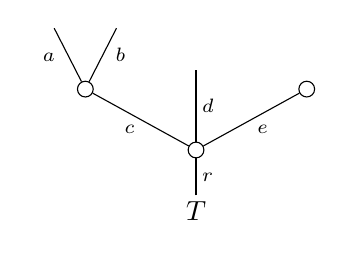
\begin{tikzpicture}[auto,grow=up, level distance = 2.2em,
	every node/.style={font=\scriptsize,inner sep = 2pt}]%
	\tikzstyle{level 2}=[sibling distance=4em]%
	\tikzstyle{level 3}=[sibling distance=2.25em]%
            \node [font=\normalsize] {$T$}
            child{node [dummy] {}
              child{node [dummy] {}
                edge from parent node [swap] {$e$}
              }
              child[level distance = 2.9
              em]{edge from parent node [swap] {$d$}}
              child{node [dummy] {}
                child{edge from parent node [near end, swap] {$b$}}
                child{edge from parent node [near end] {$\phantom{b}a$}}
                edge from parent node {$c$}
              }
              edge from parent node [swap] {$r$}
            };        
      \end{tikzpicture}
\end{equation}
Edges with no vertices $\circ$ above them are called \textit{leaves}, the unique bottom edge is called the \textit{root},
and edges that are neither are called \textit{inner edges}.
In the example above, $a$, $b$ and $d$ are leaves, $r$ is the root, and $c$ and $e$ are inner edges.
The sets of edges, inner edges, and vertices of a tree $T$ are denoted 
$\boldsymbol{E}(T)$, 
$\boldsymbol{E}^{\mathsf{i}}(T)$, 
and $\boldsymbol{V}(T)$, respectively.


While the tree diagram description above is helpful for visualizing objects in $\Omega$,
in order to describe the arrows,
we will use the algebraic notion of
a \emph{broad poset},
originally due to Weiss \cite{Wei12}
and further developed in \cite{Per18},
which we now briefly recall.
%
For each edge $t$ in a tree topped by a vertex $\circ$, we write
$t^{\uparrow}$
for the tuple of edges immediately above $t$.
In \eqref{eq:TREE} one has  
$r^{\uparrow} = cde$, 
$c^\uparrow = ab$, 
and $e^\uparrow = \epsilon$,
where $\epsilon$ denotes the empty tuple.
Each vertex can then be encoded symbolically as
$t^{\uparrow} \leq t$,
which we call a 
\emph{generating broad relation}.
This notation is motivated by a form of transitivity.
For example,
in \eqref{eq:TREE}
the relations
$cde \leq r$ and $ab \leq c$
generate, under \emph{broad transitivity},
the relation $abde \leq r$,
and one may similarly obtain relations
$cd \leq r$ and $abd \leq r$.
These relations, together with identity relations $t \leq t$,
then form the \emph{broad poset associated with $T$}.
% (alternatively, this broad poset data
% is essentially equivalent to the data of
% the colored operad $\Omega(T)$ associated to $T$ 
% (cf. \cite[\S 3]{MW07}, \cite[Rem. 4.4]{Per18}, \cite[ \eqref{TAS-TAUNER EQ}]{BP_TAS}))


A map of trees $\varphi \colon S \to T$
in $\Omega$ is then an underlying map
of edge sets 
$\varphi \colon \boldsymbol{E}(S) \to \boldsymbol{E}(T)$
which preserves broad relations.

If an edge $t$ is pictorially above (or equal to) an edge $s$, we write $t \leq_d s$.
Equivalently, $t \leq_d s$ if there exists a broad relation $s_1\dots s_n \leq s$ such that $t = s_i$ for some $i$.\\

Our discussion will be simplified by assuming 
that $\Omega$ has exactly one representative of 
each \emph{planarized tree},
by which we mean a tree together with a planar representation as in \eqref{eq:TREE}.
% (algebraically, 
% planarizations are
% suitable extensions of $\leq_d$ to a total order
% \cite[\S 3.1]{BP_geo}).
% Importantly, this implies that each map  
% $\varphi \colon S \to T$ in $\Omega$
% has a (strictly) unique factorization
% $S \xrightarrow{\simeq} S' \to T$
% as an isomorphism followed by a \emph{planar map}
% \cite[Prop. 3.24]{BP_geo}.
% Informally, $S'$ is obtained by giving $S$ the planarization ``pulled back'' from $T$.
% Note that,
In particular, the wide subcategory of $\Omega$ spanned by planar maps is skeletal,
i.e. the only planar isomorphisms are the identities.




\begin{notation}
	We write $\eta$ for the \textit{stick} tree, the unique tree with a single edge and no vertices.
\end{notation}



\begin{example}\label{TREEMAP_EX}
	The edge labels in each tree $S_i$ below determine maps
	$\boldsymbol{E}(S_i) \to \boldsymbol{E}(T)$,
	where $T$ is as in \eqref{eq:TREE}.
	For $i \leq 5$ this encodes maps
	$S_i \to T$ in $\Omega$,
	but not for $i=6$.
\begin{equation}
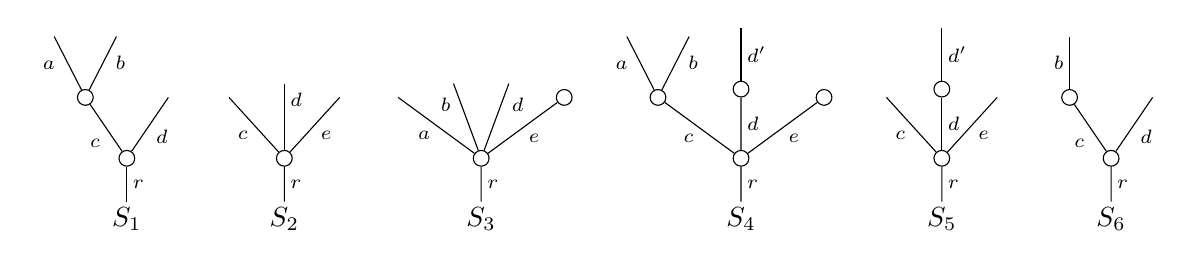
\begin{tikzpicture}[auto, grow=up, level distance = 2.2em,
	every node/.style={font=\scriptsize,inner sep = 2pt}]
\tikzstyle{level 2}=[sibling distance=3em]%
\tikzstyle{level 3}=[sibling distance=2.25em]%
	\node at (0,0) [font=\normalsize] {$S_1$} % 
                  child{node [dummy] {}
                    child{edge from parent node [swap] {$d\phantom{c}$}}
                    child{node [dummy] {}
                      child{edge from parent node [near end, swap] {$b$}}
                      child{edge from parent node [near end] {$\phantom{b}a$}}
                      edge from parent node {$\phantom{d}c$}
                    }
                    edge from parent node [swap] {$r$}
                  };
\tikzstyle{level 2}=[sibling distance=2em]%
	\node at (2,0) [font=\normalsize] {$S_2$} %
                  child{node [dummy] {}
                    child{edge from parent node [swap] {$e$}}
                    child [level distance = 2.7em] {edge from parent node [swap,near end] {$d$}}
                    child{edge from parent node {$c$}}
                    edge from parent node [swap] {$r$}
                  };
	\node at (4.5,0) [font=\normalsize] {$S_3$} 
                  child{node [dummy] {}
                    child{node [dummy] {}
                      edge from parent node [swap] {$e\phantom{a}$}
                    }
                    child [level distance = 2.7em]{edge from parent node [swap, very near end] {$d$}}
                    child [level distance = 2.7em]{edge from parent node [very near end] {$b$}}
                    child{edge from parent node {$\phantom{e}a$}}
                    edge from parent node [swap] {$r$}
                  };
                  \tikzstyle{level 2}=[sibling distance=3em]%
                  \node at (7.8,0) [font=\normalsize] {$S_4$} 
                  child{node [dummy] {}
                    child{node [dummy] {}
                      edge from parent node [swap] {$e$}
                    }
                    child[level distance = 2.5em]{node [dummy] {}
                      child[level distance = 2.2em]{edge from parent node [swap] {$d'$}}
                      edge from parent node [swap] {$d$}
                    }
                    child{node [dummy] {}
                      child{edge from parent node [swap,near end] {$b$}}
                      child{edge from parent node [near end] {$\phantom{b}a$}}
                      edge from parent node {$c$}
                    }
                    edge from parent node [swap] {$r$}
                  };
                  \tikzstyle{level 2}=[sibling distance=2em]%
                  \node at (10.35,0) [font=\normalsize] {$S_5$} %
                  child{node [dummy] {}
                    child{edge from parent node [swap] {$e$}}
                    child[level distance = 2.5em]{node [dummy] {}
                      child[level distance = 2.2em]{edge from parent node [swap] {$d'$}}
                      edge from parent node [swap] {$d$}
                    }
                    child{edge from parent node {$c$}}
                    edge from parent node [swap] {$r$}
                  };
                  \tikzstyle{level 2}=[sibling distance=3em]%
                  \node at (12.5,0) [font=\normalsize] {$S_6$}
                  child{node [dummy] {}
                    child{edge from parent node [swap] {$d\phantom{c}$}}
                    child{node [dummy] {}
                      child{edge from parent node {$b$}}
                      edge from parent node {$\phantom{d}c$}
                    }
                    edge from parent node [swap] {$r$}
                  };
\end{tikzpicture}
\end{equation}
\end{example}


\begin{definition}
        \label{TREEMAP_DEF}
        A map of trees $\varphi \colon S \to T$ is called:
        \begin{itemize}
        \item a \textit{tall map} if
                $\varphi(\underline{l}_S) = \underline{l}_T$ and $\varphi(r_S) = r_T$,
                with $\underline{l}_{(-)}$ and $r_{(-)}$ denoting the tuple of leaf edges and the root edge;
        \item a \textit{face map} if it is injective on edges;
                an \textit{inner face} if it is also tall; and
                an \textit{outer face} if, for any factorization
                $\varphi \simeq \varphi_1\varphi_2$
                with $\varphi_1,\varphi_2$ face maps
                and $\varphi_2$ inner, 
                $\varphi_2$ is an isomorphism;
                % it does not
                % admit a factorization as a non-isomorphism inner face followed by a face map;
        \item a \textit{degeneracy} if it is surjective on edges and preserves leaves
                (and is thus tall).
        \item a \textit{convex map} if whenever
                $e <_d e' <_d e''$ in $T$ 
                and $e,e''$ in the image of $\varphi$,
                then $e'$ is as well.
        \end{itemize}
\end{definition}

Pictorially, inner face maps 
$S \to T$ remove some edges in $T$
(and merge the vertices adjacent to those edges),
outer face maps remove some vertices of $T$,
and degeneracies collapse some of the unary vertices of $S$.
Tall maps are combinations of inner faces and degeneracies, while
convex maps are combinations of outer faces and degeneracies (cf. Remark \ref{TREEFACTNAMES_REM}).


\begin{example}
	In Example \ref{TREEMAP_EX},
	$S_1 \to T$ is an inner face,
	$S_2 \to T$ is an outer face,
	$S_3 \to T$ is a face that is neither inner nor outer,
	$S_4 \to T$ is a degeneracy,
        and $S_5 \to T$ is a convex map.
\end{example}


\begin{notation}\label{MAPLABELS_NOT}
	Throughout the remainder of this paper,
        we will label a 
        map in $\Omega$
        by the letters d/i/o/t/f/p
        to indicate that the map is
        a degeneracy/inner face/outer face/tall/face/planar.
\end{notation}


\begin{proposition}[{\cite[Prop. 2.2]{BP_edss}}]
      \label{TREEFACT_PROP}
      A map of trees $\varphi \colon S \to T$ % has a factorization, unique up to unique isomorphisms,
      % \begin{equation}\label{NP_TREEFACT_EQ}
      %         S \xrightarrow{d} 
      %         S' \xrightarrow{i} 
      %         S'' \xrightarrow{o}
      %         T
      % \end{equation}
      % as a degeneracy followed by an inner face followed by an outer face.
      % Accounting for planar structures, $\varphi$
      has a strictly unique factorization
      \begin{equation}\label{TREEFACT_EQ}
              S \xrightarrow{\simeq}
              S_p \xrightarrow{pd} 
              \varphi S \xrightarrow{pi} 
              \overline{\varphi S} \xrightarrow{po} T
      \end{equation}
      as an isomorphism followed by a planar degeneracy, a planar inner face, and a planar outer face.
\end{proposition}


\begin{remark}\label{TREEFACT_REM}
      The notation $\varphi S$ is motivated by the fact that this tree has edge set
      $\boldsymbol{E}(\varphi S) = \varphi (\boldsymbol{E}(S))$,
      while the 
      notation $\overline{\varphi S}$ is an instance of the 
      \emph{outer closure of an inner face}
      notation in \cite[Not. 2.14]{BP_edss}.
\end{remark}

\begin{remark}[{cf. \cite[Rem. \ref{TAS-TODF REM}, \ref{TAS-CNVXM REM}, \ref{TAS-TREEMAPCOMP_REM}]{BP_TAS}}]
        \label{TREEFACTNAMES_REM}
        We note that for any subset
	$\mathcal{S} \subseteq \{\simeq,pd,pi,po\}$
	of the arrow labels 
	in \eqref{TREEFACT_EQ},
	the type of maps whose
	factors labeled by $\mathcal{S}$ are identities 
	is closed under composition.

        In particular, as (non-planar) tall maps (resp. face maps, convex maps) can be equivalently characterized as those maps such that
        the component labeled $po$ (resp. $pd$, $pi$)
        in the decomposition \eqref{TREEFACT_EQ}
        is the identity,
        we have that these collections of maps (and their planar analogues) are closed under composition.
\end{remark}




Next, we recall the categories of colored trees used in 
\cite[Def. \ref{OC-COLFOR DEF}]{BP_FCOP}.

\begin{definition}\label{CTREE_DEF}
        Let $\mathfrak C$ be a set of colors.
        The category $\Omega_{\mathfrak C}$ of \textit{$\mathfrak C$-trees} has:
        \begin{itemize}
        \item objects pairs $\vect T = (T, \mathfrak c)$ with
                $T \in \Omega$ a tree and
                $\mathfrak c \colon \boldsymbol{E}(T) \to \mathfrak C$ a coloring of its edges;
        \item arrows $\vect S = (S, \mathfrak d) \to (T, \mathfrak c) = \vect{T}$ maps
                $\varphi \colon S \to T$ in $\Omega$ such that $\mathfrak d = \mathfrak c \varphi$.
        \end{itemize}
\end{definition}

For any map of sets $f \colon \mathfrak C \to \mathfrak D$, there is an associated functor
\begin{equation}
        \label{TREECHANGEC_EQ}
        f \colon \Omega_{\mathfrak C} \to \Omega_{\mathfrak D},
        \qquad
        \vect T = (T, \mathfrak c)
        \longmapsto
        (T, \boldsymbol{E}(T) \xrightarrow{\mathfrak c} \mathfrak C \xrightarrow{f} \mathfrak D) =: f \vect T.
\end{equation}



We end this subsection with a discussion of corollas.

\begin{definition}
        A \textit{corolla} is a tree with a single vertex.
        Similarly, a \textit{$\mathfrak C$-corolla} is
        a $\mathfrak C$-tree $\vect C = (C, \mathfrak c \colon \boldsymbol{E}(C) \to \mathfrak C)$
        whose underlying tree $C$ is a corolla.

        We record that the subcategory of $\Omega$ spanned by corollas and isomorphisms is naturally identified with
        the category $\Sigma$ of standard finite order sets $\set{1, 2, \dots, n}$ and non-ordered isomorphisms.
        We thus denote by $\Sigma_{\mathfrak C}$ the subcategory of $\Omega_{\mathfrak C}$ spanned by $\mathfrak C$-corollas and isomorphisms.        
\end{definition}

\begin{notation}
     \label{LR_NOT}
     For each $T \in \Omega$, there exists a unique corolla $\mathsf{lr}(T)$ equipped with a planar tall map
     $\mathsf{lr}(T) \to T$,
     which we call the \textit{leaf-root} of $T$.
     Explicitly, $\mathsf{lr}(T)$ has the same leaf tuple $\underline{l}_T$ and root edge $r_T$ as $T$,
     and a single vertex/generating broad relation $\underline{l}_T \leq r_T$.
     
     Similarly, for each $\mathfrak C$-tree $\vect T = (T, \mathfrak c)$,
     the $\mathfrak C$-corolla
     $\mathsf{lr}(\vect T) = (\mathsf{lr}(T), \mathfrak c_{\mathsf{lr}(T)})$,
     where $\mathfrak c_{\mathsf{lr}(T)}$ is the restriction of $\mathfrak c$ to $\boldsymbol{E}(\mathsf{lr}(T))$,
     is the unique $\mathfrak C$-corolla
     equipped with a planar tall map of $\mathfrak C$-trees $\mathsf{lr}(\vect T) \to \vect T$.

     Let $\Omega^0 \subseteq \Omega$, $\Omega_{\mathfrak C}^0 \subseteq \Omega_{\mathfrak C}$
     denote the wide subcategories spanned by the isomorphisms.
     Then the assignments $\mathsf{lr}$ extend to functors
     \[
             \mathsf{lr} \colon \Omega^0 \to \Sigma,
             \qquad
             \mathsf{lr} \colon \Omega_{\mathfrak C}^0 \to \Sigma_{\mathfrak C}.
     \]
\end{notation}


\begin{notation}
        \label{TV_NOT}
        For any tree $T$ and $v \in \boldsymbol{V}(T)$,
        we let $T_v \to T$ denote the planar outer face consisting of only this vertex and its adjacent edges.
        % Algebraically, if the vertex $v$ corresponds to the generating broad relation $e^\uparrow \leq e$,
        % then $T_v$ has edge set $e^{\uparrow} \cup \set{e}$
        % and the single broad relation $e^\uparrow \leq e$.
        
        Similarly, for any $\mathfrak C$-tree $\vect T = (T, \mathfrak c \colon \boldsymbol{E}(T) \to \mathfrak C)$
        and any vertex $v \in \boldsymbol{V}(T)$,
        we write $\vect T_v = (T_v, \mathfrak c_v)$ for the associated $\mathfrak C$-corolla,
        where $\mathfrak c_v$ is the restriction of $\mathfrak c$ to $\boldsymbol{E}(T_v) \subseteq \boldsymbol{E}(T)$. 
        \todo[inline]{can't find a similar discussion in TAS}        
\end{notation}


\subsection{Operads, and nerves}
\label{NERVE_SEC}

% The goal of this mostly expository subsection is to recall the setup and proof of Theorem \ref{SSC_THM},
% which allows us to identify simplicial operads as presheaves satisfying a strict Segal condition.
% We first recall simplicial operads and preoperads.


\subsubsection*{Simplicial operads}

We write $\sOp = \Op(\sSet)$ for the category of \textit{colored simplicial operads}, also called \textit{simplicially enriched multicategories}.
Formally, these are 
algebras over the monad $\mathbb F$ from \cite[Def. \ref{OC-FREEOP DEF}]{BP_FCOP}
in the category $\Sym_\bullet(\sSet)$ of \textit{colored symmetric sequences}.

For this paper, it suffices to give \todo{the shortest description possible} an explicit description:
a simplicial operad $\O \in \sOp$ with color set $\mathfrak C$
has levels $\O(\vect C)$ indexed by
$\mathfrak C$-corollas $\vect C$, % $ = (C, \mathfrak c \colon \boldsymbol{E}(C) \to \mathfrak C)$,
and composition laws induced by $\mathfrak C$-colored trees:
for each $\mathfrak C$-tree $\vect T$,
there are unital and associative maps
\[
        \prod_{v \in \boldsymbol{V}(T)}\O(\vect T_v) \longto \O(\mathsf{lr}(\vect T)),
\]
natural in $\vect T$.
A map
$\phi \colon \O \to \P$
in the category $\sOp_{\mathfrak C}$ of \textit{$\mathfrak C$-colored operads}
is then given by a collection of natural maps
$\phi(\mathfrak C) \colon \O(\mathfrak C) \to \P(\mathfrak C)$,
such that the associated diagrams of composition laws commute.

For any map of sets $f \colon \mathfrak D \to \mathfrak C$,
one has a functor (really an adjunction \cite[Rem. \ref{OC-OP_MAP REM}]{BP_FCOP})
\[
        f^{\**} \colon \sOp_{\mathfrak C} \to \sOp_{\mathfrak D},
        \qquad
        f^{\**}\O(\vect C) = \O(f \vect C)
        % \hat{f}_! \colon \sOp_{\mathfrak D} \rightleftarrows \sOp_{\mathfrak C} \colon f^{\**}
\]
with $f \vect C$ as in \eqref{TREECHANGEC_EQ}.
% while the left adjoint is the less explicit
% $f_! \O = \mathop{coeq}\left( \mathbb F(f_! \mathbb F \O) \rightrightarrows \mathbb F f_! \O\right)$.


\begin{definition}
        The category $\sOp$ of \textit{colored simplicial operads}
        has objects $(\O, \mathfrak C)$ where $\O$ is a $\mathfrak C$-colored operad,
        and arrows $(\O, \mathfrak C) \to (\P, \mathfrak D)$ given by pairs $(F,f)$
        where $f \colon \mathfrak C \to \mathfrak D$ is a map of sets and
        $F \colon \O \to f^{\**}\P$ is a map of $\mathfrak C$-colored operads.
\end{definition}


\begin{example}
        One important class of colored operads are the free operads generated by trees.
        Given $T \in \Omega$, we define $\Omega(T)$ to be the $\boldsymbol{E}(T)$-colored operad which,
        when evaluated on an $\boldsymbol{E}(T)$-colored corolla
        $\vect C = (C, \mathfrak c \colon \boldsymbol{E}(C) \to \boldsymbol{E}(T))$, is given by
        \begin{equation}\label{OMEGADEF_EQ}
                \Omega(T)(\vect C) =
                \begin{cases}
                        \** \qquad & 
                        \mbox{if
                          $\mathfrak{c} \colon \boldsymbol{E}(C) \to \boldsymbol{E}(T)$
                          defines a map $C \to T$ in $\Omega$}
                        \\
                        \varnothing & \text{otherwise.}
                \end{cases}
        \end{equation}
        Note that, as the levels of $\Omega(T)$ are $\**$ or $\varnothing$,
        one has at most one way to compose operations,
        and thus there exists at most one possible operad structure on $\Omega(T)$.
        That this structure exists
        (i.e. that composition is well defined)
        follows since,
        for any other tree $S \in \Omega$,
        a coloring
        $\mathfrak{c} \colon \boldsymbol{E}(S) \to \boldsymbol{E}(T)$
        defines a map
        $S \to T$ in $\Omega$
        iff
        the restrictions
        $\mathfrak{c}_v \colon \boldsymbol{E}(S_v) \to \boldsymbol{E}(T)$
        define maps
        $S_v \to T$ in $\Omega$
        for all vertices $v \in \boldsymbol{V}(S)$.
\end{example}


\subsubsection*{Dendroidal sets and preoperads}

We recall simplicial dendroidal sets and preoperads.
An extensive discussion can be found in
e.g. \cite[\S 4]{BP_edss}, \cite[\S \ref{TAS-JT_SEC}, \S \ref{TAS-SPREOP_SEC}]{BP_TAS}.

% We will identify simplicial oeprads with their nerves below. 
% (Simplicial) operads can also be identified as presheaves satisfying a strict Segal condition,
% under the \textit{nerve} construction (Theorem \ref{SSC_THM} below).
% As this perspective is quite helpful,
% we briefly discuss this connection now.

% Recall that the nerve functor
% $N \colon \Cat \to \sSet$
% sends a category $\mathcal C$ to the simplicial set $N \mathcal C$
% $N \mathcal C_n = \Hom([n], \mathcal C)$,
% where $[n] = \set{0 \to 1 \to \dots \to n}$.
% %
% Similarly, the \textit{dendroidal nerve} functor
% \begin{equation}
%         \label{OPN_EQ}
%         N \colon \Op \to \dSet
% \end{equation}
% sends an operad $\O$ to the dendroidal set defined on $T \in \Omega$ by
% $N \O(T) = \Hom(\Omega(T), \O)$,
% with $\Omega(T)$ as in \eqref{OMEGADEF_EQ}.

% This functor extends by postcomposition to the associated categories of simplicial presheaves,
% yielding the left functor below,
% \begin{equation}
%         \label{SOPN_EQ}
%         N^{\Delta^{op}} \colon \Op^{\Delta^{op}} \to \sdSet,
%         \qquad
%         N \colon \sOp \to \PreOp,
% \end{equation}
% where $\sdSet = \Set^{\Delta^{op} \times \Omega^{op}}$ is the category of \textit{simplicial dendroidal sets}.
% This extension restricts to the right functor in \eqref{SOPN_EQ},
% using the inclusions
% \[
%         \sOp \hookrightarrow \Op^{\Delta^{op}},
%         \qquad
%         \mathsf{PreOp} \hookrightarrow \sdSet,
% \]
% regarding simplicially enriched operads as simplicial objects in operads whose
% structure maps are all the identity on the set of colors,
% and where $\mathsf{PreOp}$ is the full subcategory of \textit{preoperads},
% those $X \in \sdSet$ such that $X(\eta)$ is a discrete simplicial set.


Let $\dSet = \Set^{\Omega^{op}}$ and $\sdSet = \Set^{\Delta^{op} \times \Omega^{op}}$
denote the categories of \textit{dendroidal sets} and \textit{simplicial dendroidal sets}.

\begin{definition}
        For $T \in \Omega$, let $\Omega[T] \in \dSet$ denote the \textit{representable} dendroidal set
        $\Omega[T](S) = \Omega(S,T)$.
        %
        Let $Sc[T] \subseteq \Omega[T]$ denote the \textit{Segal core} of $T$, given by
        \[
                Sc[T] = \bigcup_{U \in \mathsf{Face}_{sc}(T)} \Omega[U],
        \]
        where
        $\mathsf{Face}_{sc}(T)$ is the poset of planar outer faces of $T$ with no inner edges
        (i.e. $U$ is either a single edge or a single vertex)
        and the union takes place in $\Omega[U]$.
\end{definition}

\begin{notation}
        For $X \in \sdSet$, we write $X_n(T)$ for the evaluation at $n \in \Delta$ and $T \in \Omega$,
        and refer to $n$ and $T$ as the \textit{simplicial} and \textit{dendroidal} directions, respectively.
        %
        More generally, for $X \in \sdSet$ we write
        \begin{equation}
                \label{SDSET_EQ}
                % X_{(-)} \colon \sSet \to \dSet^G,
                % \qquad
                X(-) \colon \dSet \to \sSet,
                \qquad
                X(A)_n = X_n(A) = \dSet(A, X_n),
        \end{equation}
        for the unique (up to unique natural isomorphism) colimit-preserving functor
        such that
        % $X_{\Delta[n]} = X_n$ and 
        $X\left(\Omega[U]\right) = X(U)$ for
        % $n \geq 0$,
        $U \in \Omega$.
        % Explicitly, % $X_K(U) = \sSet(K, X(U))$ and
        % $X(A)_n = \dSet(A, X_n)$.
        % \item Given $X \in \sdSet$, we write $\sk_\eta X \in \sdSet$ for the \textit{skeleton}, given by
        %         \[
        %                 (\sk_\eta X)(U) = \coprod_{\boldsymbol{E}(U)} X(\eta).
        %         \]
\end{notation}

\begin{definition}
        Let $\PreOp \subseteq \sdSet$ denote the full subcategory spanned by the \textit{preoperads},
        those $X \in \sdSet$ such that $X(\eta)$ is a discrete simplicial set.

        For $X \in \PreOp$, we call $X(\eta)$ the \textit{color set} of $X$.
\end{definition}

\begin{notation}
        Given $X \in \PreOp$, $T \in \Omega$, and a coloring $\mathfrak c \colon \boldsymbol{E}(T) \to X(\eta)$,
        we define $X_{\mathfrak c}(T) \in \sSet$ as the pullback below.
        \begin{equation}
                \label{XUDECALT EQ}
                \begin{tikzcd}
                        X_{\mathfrak c}(T) \arrow[r] \arrow[d]
                        &
                        X(T) \arrow[d]
                        \\
                        \** \arrow[r, "\mathfrak c"]
                        &
                        \displaystyle{
                          \prod\limits_{\boldsymbol{E}(T)} X(\eta)
                        }
                \end{tikzcd}
        \end{equation}
\end{notation}

\begin{remark}
        For any $X$, $T$, $\mathfrak c$ as in \eqref{SDSET_EQ} % in Notation \ref{PREOP_NOT}\ref{XUC_LBL},
        we have a coproduct decomposition \cite[ \eqref{TAS-COLDEC_EQ}]{BP_TAS}
        \begin{equation}
                \label{COLDEC_EQ}
                X(T) \simeq \coprod_{\mathfrak c \colon \boldsymbol{E}(T) \to X(\eta)} X_{\mathfrak c}(T).
        \end{equation}
        Moreover, $X_{\mathfrak c}(T)$ is natural in $(T, \mathfrak c) \in \Omega_{\mathfrak C}^{op}$
        and in fact
        $X$ is determined by the presheaf $(T, \mathfrak c) \mapsto X_{\mathfrak c}(T)$
        (cf. \cite[ \eqref{TAS-PREOPCOLFIXEQ EQ}]{BP_TAS}).
        % \begin{proposition}[{cf. \cite[ \eqref{TAS-PREOPCOLFIXEQ EQ}]{BP_TAS}}]
        %         There is an equivalence of categories
        %         \[
        %                 \PreOp_{\mathfrak C} \to \Fun_{\**}(\Omega_{\mathfrak C}^{op}, \sSet),
        %                 \qquad
        %                 \big(T \mapsto X(T)\big) \mapsto \big( (T, \mathfrak c) \mapsto X_{\mathfrak c}(T) \big)
        %         \]
        %         where $\Fun_{\**}(\Omega_{\mathfrak C}^{op}, \sSet) \subseteq \Fun(\Omega_{\mathfrak C}^{op}, \sSet)$
        %         is the subcategory spanned by those functors $Y$ such that $Y(\eta, \mathfrak c) = \**$ for all colorings of the stick tree $\eta$.
        % \end{proposition}
        
        Henceforth, we will work with the $X_{\mathfrak c}(T)$ notation as the levels of our preoperads.
\end{remark}


\begin{remark}[{cf. \cite[ (\ref{TAS-STRSEGCON EQ})]{BP_TAS}}]
        \label{NERVEEVAL_REM}
        Given a $\mathfrak C$-colored operad $\O \in \sOp$, using the notation from \eqref{XUDECALT EQ} we have
        \[
                N\O_{\mathfrak c}(C) = \O(\vect C),
                \qquad
                N \O_{\mathfrak c}(T) = \prod_{v \in \boldsymbol{V}(T)} \O(T_v, \mathfrak c_v).
        \]
        for all $\mathfrak C$-corollas $\vect C = (C, \mathfrak c)$ and
        $\mathfrak C$-trees $\vect T = (T, \mathfrak c)$.
        % 
        % In particular, $\Omega[T] = N\Omega(T)$ (cf. \cite[Rem. \ref{TAS-NERVESIMDES REM}]{BP_TAS}).
\end{remark}

\subsubsection*{The strict Segal condition and the nerve}

% We now define the strict Segal condition.

\begin{definition}
        \label{SSC_DEF}
        We say $X \in \PreOp$ satisfies the \textit{strict Segal condition} if
        the Segal maps
        \begin{equation}
                \label{SSC_EQ}
                X_{\mathfrak c}(T) \xrightarrow{\simeq} \prod_{v \in \boldsymbol{V}(T)} X_{\mathfrak c_v}(T_v)
        \end{equation}
        (induced by the inclusions $\vect T_v \hookrightarrow \vect T$)
        are isomorphisms of simplicial sets
        for all $T \in \Omega$ and colorings $\mathfrak c \colon \boldsymbol{E}(T) \to X(\eta)$.
\end{definition}

\begin{remark}
        \label{SSC_REM}
        This strict Segal condition is equivalent to the following conditions,
        where we note that condition (i) is the description given in \cite{MW09} and \S \ref{MAINRESULT_SEC}.        
        \begin{enumerate}
        \item $X_n$ has the strict right lifting property against
                the inner horn inclusions $\Lambda^e[T] \to \Omega[T]$,
                for all $T \in \Omega$, and inner edge $e \in \boldsymbol{E}^i(T)$, and $n \geq 0$.
        \item The maps $X(T) \to X(\Lambda^e[T])$
                are isomorphisms of simplicial sets,
                for all $T \in \Omega$
        \item $X_n$ has the strict right lifting property against
                the Segal core inclusions $Sc[T] \to \Omega[T]$,
                for all $T \in \Omega$ and $n \geq 0$.
        \item The maps
                $X(T) \to X(Sc[T])$
                are isomorphisms of simplicial sets,
                for all $T \in \Omega$.
        \end{enumerate}
        Here,
        % $\Omega[T] \in \dSet$ denotes the \textit{representable} dendroidal set,
        $\Lambda^e[T] \subseteq \Omega[T]$ denotes the \textit{inner horn} of $T$ associated to the inner edge $e$
        % $Sc[T] \subseteq \Omega[T]$ denotes the \textit{Segal core} of $T$
        (cf. \cite[\S 2]{CM13a}, \cite[\S 2.3]{BP_edss}).
        In Definition \ref{SSC_DEF},
        We regard $\Omega[T]$, $\Lambda^e[T]$, and $Sc[T]$
        as preoperads using the constant/evaluation adjunction 
        \[
                c_! \colon \dSet \rightleftarrows \sdSet \colon (-)_0,
                \qquad
                (c_!A)_n(T) = A_n,
                \quad
                (X_0)(T) = X_0(T),
        \]
        % given by the dendroidally-constant presheaf $(c_!A)_n(T) = A_n$
        % and the evaluation at 0 presheaf $(X_0)(T) = X_0(T)$,
        as $c_!$ is fully-faithful.
        
        Indeed,
        (i) iff (ii) and (iii) iff (iv) follow by \eqref{SDSET_EQ},
        (i) iff (iii) and (ii) iff (iv) follow by either \cite[Prop. 2.5 and Cor. 2.6]{CM13a} or \cite[Props. 3.22, 3.31]{BP_edss}, and
        (iv) is equivalent to Definition \ref{SSC_DEF} by \eqref{XUDECALT EQ} and \eqref{COLDEC_EQ}.

        In particular, the essential image of $N \colon \sOp \to \PreOp$ is precisely those $X \in \PreOp$ satisfying the strict Segal condition \eqref{SSC_EQ}.

        % ---------- taken care of in introduction ----------
        % While we will exclusively use the description from Definition \ref{SSC_DEF} in this paper,
        % the conditions above are closer to the original discussions of
        % \textit{Segal operads} (and \textit{$\infty$-operads})
        % in the model structures on $\sdSet$ (and $\dSet$),
        % cf. \cite[Cor. 5.6]{CM13a}, \cite[Prop. 5.3]{BP_edss}.
\end{remark}


% \begin{definition}
%         \label{SSC_DEF}
%         We say $X \in \PreOp$ satisfies the \textit{strict Segal condition} if
%         any of the following equivalent conditions hold:
%         \begin{enumerate}
%         \item $X_n$ has the strict right lifting property against
%                 the inner horn inclusions $\Lambda^e[T] \to \Omega[T]$,
%                 for all $T \in \Omega$, and inner edge $e \in \boldsymbol{E}^i(T)$, and $n \geq 0$.
%         \item The maps $X(T) \to X(\Lambda^e[T])$
%                 are isomorphisms of simplicial sets,
%                 for all $T \in \Omega$
%         \item $X_n$ has the strict right lifting property against
%                 the Segal core inclusions $Sc[T] \to \Omega[T]$,
%                 for all $T \in \Omega$ and $n \geq 0$.
%         \item The maps
%                 $X(T) \to X(Sc[T])$
%                 are isomorphisms of simplicial sets,
%                 for all $T \in \Omega$.
%         \item The Segal maps
%                 $X_{\mathfrak c}(T) \to \prod_{v \in \boldsymbol{V}(T)} X_{\mathfrak c_v}(T_v)$
%                 are isomorphisms of simplicial sets,
%                 for all $T \in \Omega$ and colorings $\mathfrak c \colon \boldsymbol{E}(T) \to X(\eta)$.
%         \end{enumerate}
% \end{definition}


% Here,
% $\Omega[T] \in \dSet$ denotes the \textit{representable} dendroidal set,
% $\Lambda^e[T] \subseteq \Omega[T]$ denotes the \textit{inner horn} of $T$ associated to the inner edge $e$, and
% $Sc[T] \subseteq \Omega[T]$ denotes the \textit{Segal core} of $T$
% (cf. \cite[\S 2]{CM13a}, \cite[\S 2.3]{BP_edss}).
% In Definition \ref{SSC_DEF}, we regard these as preoperads using the constant/evaluation adjunction 
% \[
%         c_! \colon \dSet \rightleftarrows \sdSet \colon (-)_0,
%         \qquad
%         (c_!A)_n(T) = A_n,
%         \quad
%         (X_0)(T) = X_0(T),
% \]
% % given by the dendroidally-constant presheaf $(c_!A)_n(T) = A_n$
% % and the evaluation at 0 presheaf $(X_0)(T) = X_0(T)$,
% as $c_!$ is fully-faithful.

% \begin{remark}    
%         The above conditions are in fact all equivalent:
%         (i) iff (ii) and (iii) iff (iv) follow by \eqref{SDSET_EQ},
%         (i) iff (iii) and (ii) iff (iv) follow by either \cite[Prop. 2.5 and Cor. 2.6]{CM13a} or \cite[Props. 3.22, 3.31]{BP_edss}, and
%         (iv) iff (v) follows by \eqref{XUDECALT EQ} and \eqref{COLDEC_EQ}. 
% \end{remark}

% \begin{remark}
%         In this paper, we will only use description (v).
%         However, (i)-(iv) are closer to the original discussions of
%         \textit{Segal operads} (and \textit{$\infty$-operads})
%         in the model structures on $\sdSet$ (and $\dSet$),
%         cf. \cite[Cor. 5.6]{CM13a}, \cite[Prop. 5.3]{BP_edss}.
% \end{remark}

{\color{red}I see no reason why the nonsense below is needed.
Or most of the nonsense above. What's the point of this crap?}
{\color{blue}
  Because at no point in TAS do we actually say what we mean by the strict Segal condition in $\PreOp$,
  and the one you give in the intro is not the same as what is used in \S 3,
  nor do we observe that $N \colon \sOp \to \PreOp$ has the properties we want [though this is corrected in your introduction],
  nor do we observe that the notation behaves as in Remark \ref{NERVEEVAL_REM}, obvious as it may be.
  
  In any case, much of this can be removed due to the more  introduction.}


{\color{pink} 

% Now, recall that the nerve functor
% $N \colon \Cat \to \sSet$
% sends a category $\mathcal C$ to the simplicial set
% $N \mathcal C_n = \Hom([n], \mathcal C)$,
% where $[n] = \set{0 \to 1 \to \dots \to n}$.
% %
% Similarly, the \textit{dendroidal nerve} is given by
% \begin{equation}
%         \label{OPN_EQ}
%         N \colon \Op \to \dSet,
%         \qquad
%         N\O(T) = \Hom(\Omega(T), \O),
% \end{equation}
% % sends an operad $\O$ to the dendroidal set defined on $T \in \Omega$ by
% % $N \O(T) = \Hom(\Omega(T), \O)$,
% with $\Omega(T)$ as in \eqref{OMEGADEF_EQ}.

%   The dendroidal nerve $N$ from \eqref{SOPDSET_EQ}
%   extends by postcomposition to the associated categories of simplicial presheaves,
%   yielding the left functor below,
% \begin{equation}
%         \label{SOPN_EQ}
%         N^{\Delta^{op}} \colon \Op^{\Delta^{op}} \to \sdSet,
%         \qquad
%         N \colon \sOp \to \PreOp.
% \end{equation}
% This $N^{\Delta^{op}}$ restricts to the right functor in \eqref{SOPN_EQ}
% using the inclusions
% $\sOp \hookrightarrow \Op^{\Delta^{op}}$,
% where we regard simplicially operads as those simplicial objects in operads whose
% structure maps are all the identity on the set of colors,
% and $\mathsf{PreOp} \hookrightarrow \sdSet$.



% \begin{theorem}
%         \label{SSC_THM}
%         The nerve functor $N \colon \sOp \to \PreOp$
%         is fully-faithful, with essential image
%         those preoperads $X$ satisfying the strict Segal condition.
% \end{theorem}
% \begin{proof}
%         By \cite[Prop. 5.3 and Thm. 6.1]{MW09},
%         the nerve functor
%         $N \colon \Op \to \dSet$
%         is fully faithful, with essential image
%         those $A \in \dSet$ with the strict right lifting property against all inner horn inclusions $\Lambda^e[T] \to \Omega[T]$.
%         This implies $N^{\Delta^{op}}$ is fully-faithful, and moreover
%         the essential image of $N^{\Delta^{op}} \colon \Op^{\Delta^{op}} \to \sdSet$ is precisely
%         those $X \in \sdSet$ satisfying the strict Segal condition from Remark \ref{SSC_REM}(i).
%         % (one direction is immediate; for the other, we need that if $X$ is levelwise in the image of the nerve functor,
%         % then all the simplicial structure maps are in fact maps of operads by fully-faithfullness).
%         Restricting the source to $\sOp \hookrightarrow \Op^{\Delta^{op}}$, we may restrict the target to $\PreOp \hookrightarrow \sdSet$,
%         in which case Remark \ref{SSC_REM}(i) is equivalent to the strict Segal condition from Definition \ref{SSC_DEF}.
% \end{proof}


% \begin{remark}[{cf. \cite[ (\ref{TAS-STRSEGCON EQ})]{BP_TAS}}]
%         \label{NERVEEVAL_REM}
%         Given a $\mathfrak C$-colored operad $\O \in \sOp$, using the notation from \eqref{XUDECALT EQ} we have
%         \[
%                 N\O_{\mathfrak c}(C) = \O(\vect C),
%                 \qquad
%                 N \O_{\mathfrak c}(T) = \prod_{v \in \boldsymbol{V}(T)} \O(T_v, \mathfrak c_v).
%         \]
%         for all $\mathfrak C$-corollas $\vect C = (C, \mathfrak c)$ and
%         $\mathfrak C$-trees $\vect T = (T, \mathfrak c)$.
%         % 
%         In particular, $\Omega[T] = N\Omega(T)$ (cf. \cite[Rem. \ref{TAS-NERVESIMDES REM}]{BP_TAS}).
% \end{remark}


% \begin{remark}
% 	One neat feature of the description in 
% 	\eqref{WU_EQ}
% 	is that the nerve $N W(U)$
% 	can be defined identically 
% 	(cf. Definition \ref{NWTNS DEF}; 
% 	compare with \cite[Rem. \ref{TAS-NERVESIMDES REM}]{BP_TAS}).
% %	It is then straightforward to check that the nerve thus defined has the required functoriality and satisfies the strict Segal condition.
% %	allowing us to deduce many properties of $W_!$
% %	via systematic use of 
% %	Proposition \ref{TREEFACT_PROP}.
% 	As an aside, one can verify directly that
% 	Definition \ref{NWTNS DEF}
% 	defines a preoperad satisfying the strict Segal condition,
% 	thereby inducing the operad structure on $W(U)$.
% \end{remark}


}



\section{The dendroidal $W_!$-construction}
\label{WCONS AP}


Our discussion of the dendroidal $W_!$-construction
will make systematic
use of the factorizations in $\Omega$ given by 
Proposition \ref{TREEFACT_PROP}.
We follow Notation \ref{MAPLABELS_NOT},
and label 
a map in $\Omega$
by either of the letters d/i/o/t/f/p
to indicate that the map is
a degeneracy/inner face/outer face/tall/face/planar.

\begin{notation}
        Given a map $\phi\colon S \to T$,
        we write
        \[
                S \xrightarrow{d}
                \phi S \xrightarrow{i,p}
                \overline{\phi S} \xrightarrow{o,p}
                T
        \]
        for the (strictly) unique 
        factorization of $\phi$ with the indicated properties
        (cf. \ref{TREEFACT_EQ}).
\end{notation}
% We note that the notation 
% $\phi(S)$ is motivated by the fact that this tree has edge set
% $\boldsymbol{E}(\phi S) = \phi (\boldsymbol{E}(S))$
% while the 
% $\overline{\phi S}$ notation is an instance of the 
% \emph{outer closure of an inner face}
% notation in \cite[Not. 2.14]{BP_edss}.


We now define the notion of dendroidal necklace,
generalizing the key notion in \cite{DS11}.
 

\begin{definition}[{cf. \cite[\S 3]{DS11}}]
        \label{NECKLACE_DEF}
	A \emph{necklace} is 
	a planar inner face map
	$\mathfrak{n} \colon J \to T$
	in $\Omega$.
	Moreover:
	%
	\begin{enumerate}[label = (\roman*)]
		\item 
		$J$ is called the \emph{inner face of joints} of the necklace;
		\item for each vertex $v \in \boldsymbol{V}(J)$,
		the outer face
		$\overline{\mathfrak{n} J_v} = T_v \hookrightarrow T$
		is called a \emph{bead} of the necklace.
	\end{enumerate}
\end{definition}

\begin{example}
      \label{NECKLACE_EX}
      Consider the trees $J$ and $T$ below.
      The labeling of the edges indicates a map $\boldsymbol{E}(J) \to \boldsymbol{E}(T)$ which
      encodes an inner face map.
      \begin{equation}
            \begin{tikzpicture}[auto,grow=up, level distance = 2.2em,
                  every node/.style={font=\scriptsize,inner sep = 2pt}]%
                  \tikzstyle{level 2}=[sibling distance=4em]%
                  \tikzstyle{level 3}=[sibling distance=2.25em]%
                  \node at (-5,0) [font=\normalsize] {$J$}
                  child{node [dummy,label=-120:$v$] {}
                    child{edge from parent node [swap] {$e$}
                    }
                    child{edge from parent node [swap] {$d$}}
                    child{node [dummy,label=left:$u$] {}
                      child{edge from parent node [near end] {$a$}} %{$\phantom{b}a$}
                      edge from parent node {$c$}
                    }
                    edge from parent node [swap] {$r$}
                  };        
                  \node [font=\normalsize] {$T$}
                  child{node [dummy] {}
                    child{node [dummy] {}
                      child{edge from parent node [swap] {$e$}}
                      edge from parent node [swap] {$f$}
                    }
                    child{edge from parent node [swap] {$d$}}
                    child{node [dummy] {}
                      child{node [dummy] {}
                        edge from parent node [near end, swap] {$b$}}
                      child{edge from parent node [near end] {$\phantom{b}a$}}
                      edge from parent node {$c$}
                    }
                    edge from parent node [swap] {$r$}
                  };        
            \end{tikzpicture}
      \end{equation}
      Here, $J = T - \set{b,f}$, and the two beads are
           \begin{equation}
            \begin{tikzpicture}[auto,grow=up, level distance = 2.2em,
                  every node/.style={font=\scriptsize,inner sep = 2pt}]%
                  \tikzstyle{level 2}=[sibling distance=4em]%
                  \tikzstyle{level 3}=[sibling distance=2.25em]%
                  \node at (-5,0) [font=\normalsize] {$\overline{\mathfrak n J_u} = T_u$}
                  child{node [dummy] {}
                    child{node [dummy] {}
                      edge from parent node [near end, swap] {$b$}
                    }
                    child{edge from parent node [near end] {$\phantom{b}a$}}
                    edge from parent node [swap] {$c$}
                  };
                  \node [font=\normalsize] {$\overline{\mathfrak n J_v} = T_v$}
                  child{node [dummy] {}
                    child{node [dummy] {}
                      child{edge from parent node [swap] {$e$}}
                      edge from parent node [swap] {$f$}
                    }
                    child{edge from parent node [swap] {$d$}}
                    child{edge from parent node {$c$}}
                    edge from parent node [swap] {$r$}
                  };        
            \end{tikzpicture}
      \end{equation}
\end{example}

In the following, we write 
$\mathsf{Face}_{sc}(J)$ for the \emph{Segal core poset} of $J$,
consisting of those planar outer faces with no inner edges
(which consist of either a single edge or a single vertex of $J$).



\begin{definition}
        \label{NECKREP_DEF}
	Given a necklace $\mathfrak{n} \colon J \to T$ 
	we define its representable presheaf
	$\Omega[\mathfrak{n}] \in \mathsf{dSet}$ by
	\begin{equation}
	\Omega[\mathfrak{n}] 
	= 
	\underset{U \in \mathsf{Face}_{sc}(J)}{\colim}
	\Omega[\overline{\mathfrak{n} U}]
	=
	\bigcup_{U \in \mathsf{Face}_{sc}(J)} 
	\Omega[\overline{\mathfrak{n} U}]
	\end{equation}
	where the union formula is taken inside $\Omega[T]$.
	
	The category $\mathsf{Nec}$ of necklaces is then the full subcategory of $\mathsf{dSet}$
	spanned by the $\Omega[\mathfrak{n}]$.
\end{definition}



\begin{remark}
	The $\Omega[\mathfrak{n}]$ presheaves
	interpolate between the usual 
	Segal core and representable presheaves.
	More explicitly,
	each tree $T \in \Omega$
	gives rise to necklaces
	$T \xrightarrow{=} T$ and
	$\mathsf{lr}(T) \to T$
	for which
        \[
                \Omega[T \xrightarrow{=} T] = Sc[T],
                \qquad
                \Omega[\mathsf{lr}(T)] = \Omega[T].
        \]
        In particular,
        one obtains a natural inclusion
        $\Omega \subset \mathsf{Nec}$
        given by $T \mapsto \left( \mathsf{lr}(T) \to T \right)$.
        % 
        However, we caution that the assignment
        $T \mapsto Sc[T]$ is not functorial on $T$
        (more precisely, it is functorial only with respect to \emph{convex} maps of trees,
        in the sense of Definition \ref{TREEMAP_DEF}). % Remark \ref{TREEFACTNAMES_REM}. %\ref{CNVXM REM}).
\end{remark}



\begin{remark}
	In the context of linear trees,
	a necklace is an injective map
	$\mathfrak{n} \colon [n] \to [m]$,
	with beads $[m_i], 1 \leq n$
	such that $m_1 + \dots + m_k = m$.
	One then has an identification
	$\Omega[\mathfrak n] =
	\iota_!(\Delta[m_1] \vee \dots \vee \Delta[m_k])$
	where each $\vee$ symbol
	indicates that the last edge of 
	$\Delta[m_i]$ is identified with the first edge of
	$\Delta[m_{i+1}]$,
	thus recovering the original definition of necklace 
	due to Dugger-Spivak \cite[\S 1]{DS11}.
\end{remark}



\begin{lemma}\label{FACEINNECK LEM}
	Let $\mathfrak{n} \colon J \to T$ be a necklace. Then
	\begin{enumerate}[label=(\roman*)]
		\item a face $U \hookrightarrow T$
		is in $\Omega[\mathfrak{n}]$
		iff its outer closure $\bar{U}$ is; 
		\item an outer face 
		$U = \bar{U} \hookrightarrow T$
		is in $\Omega[\mathfrak{n}]$ iff 
		$\boldsymbol{E}^{\mathsf{i}}(J) \cap 
		\boldsymbol{E}^{\mathsf{i}}(U) = \emptyset$;
		\item there is a decomposition
		$
		\boldsymbol{E}(T) = 
		\boldsymbol{E}(J) \amalg 
		\coprod_{v \in \boldsymbol{V}(J)}
		\boldsymbol{E}^{\mathsf{i}}(T_v)
		$.
	\end{enumerate}
\end{lemma}



\begin{proof}
	(i) follows since $\Omega[\mathfrak{n}]$ is an union of outer faces.
	
	The arguments for (ii),(iii) are by induction on the number of inner edges $\boldsymbol{E}^{\mathsf{i}}(J)$,
	with the base case of $\boldsymbol{E}^{\mathsf{i}}(J) = \emptyset$  being obvious.
%	
	Otherwise, letting $e \in \boldsymbol{E}^{\mathsf{i}}(J)$, since $e$ is an inner edge of
	both $J$ and $T$
	one has grafting decompositions
	$J = J' \amalg_e J''$,
	$T = T' \amalg_e R''$
	together with inner face maps
	$\mathfrak{n}' \colon J' \to T'$,
	$\mathfrak{n}'' \colon J'' \to T''$.
%
	One then has that 
	$U$ is in $\Omega[\mathfrak{n}]$
	iff it is in either
	$\Omega[\mathfrak{n}']$ or in $\Omega[\mathfrak{n}'']$,
	yielding the induction step for (ii).
	The induction step for (iii) likewise follows. 
\end{proof}



\begin{remark}
	If $S \xrightarrow{d} S'$
	is a degeneracy,
	the vertices of $S'$ are naturally identified with
	the vertices of $S$ that are not collapsed to edges.
	Thus, by factoring a tall map
	$\varphi \colon S \xrightarrow{t} T$ as
	$S \xrightarrow{d} \varphi S \xrightarrow{i} T$
	the decomposition (iii) in Lemma \ref{FACEINNECK LEM}
	generalizes to 
\begin{equation}\label{EDGEBREAK EQ}
	\boldsymbol{E}(T) = 
	\boldsymbol{E}(\varphi S) \amalg 
	\coprod_{v \in \boldsymbol{V}(S)}
	\boldsymbol{E}^{\mathsf{i}}(\overline{\varphi S_v}).
\end{equation}
\end{remark}



\begin{notation}
	Given a necklace
	$\mathfrak{n} \colon J \to T$
	and outer face $F \to T$
	we write 
	$\mathfrak{n}_F \colon J_F \to F$
	for the necklace characterized by
\[
	\boldsymbol{E}^{\mathsf{i}}(J_F)
	=
	\boldsymbol{E}^{\mathsf{i}}(J)
	\cap
	\boldsymbol{E}^{\mathsf{i}}(F).
\]
\end{notation}

\begin{example}
      Let $\mathfrak n \colon J \to U$ be the necklace in Example \ref{NECKLACE_EX},
      and consider the outer faces $F$ and $F'$ of $T$ depicted below.
      Then $J_F$ is as depicted and $J_{F'} = F'$.
\begin{equation}
\begin{tikzpicture}[auto,grow=up, level distance = 2.2em,
                  every node/.style={font=\scriptsize,inner sep = 2pt}]%
\tikzstyle{level 2}=[sibling distance=4em]%
\tikzstyle{level 3}=[sibling distance=2.25em]%
	\node at (-10,0) [font=\normalsize] {$F$}
                  child{node [dummy] {}
                    child{node [dummy] {}
                      child{edge from parent node [swap] {$e$}}
                        edge from parent node [swap] {$f$}
                    }
                    child{edge from parent node [swap] {$d$}}
                    child{edge from parent node {$c$}}
                    edge from parent node [swap] {$r$}
                  };
	\node at (-5,0) [font=\normalsize] {$J_F$}
                  child{node [dummy] {}
                    child{edge from parent node [swap] {$e$}}
                    child{edge from parent node [swap] {$d$}}
                    child{edge from parent node {$c$}}
                    edge from parent node [swap] {$r$}
                  };     
	\node [font=\normalsize] {$F' = J_{F'}$}
                  child{node [dummy] {}
                    child{edge from parent node [swap] {$f$}}
                    child{edge from parent node [swap] {$d$}}
                    child{node [dummy] {}
                      child{edge from parent node [swap, near end] {$b$}}
                      child{edge from parent node [near end] {$a$}} % {{$\phantom{b}a$}}
                      edge from parent node {$c$}
                    }
                    edge from parent node [swap] {$r$}
                  };
\end{tikzpicture}
\end{equation}
In particular, note that one need not have a map $J_F \to J$
since $\boldsymbol{E}(J)$
may not contain $\boldsymbol{E}(J_F)$.
\end{example}



\begin{corollary}\label{NECINT COR}
	Let $\mathfrak{n} \colon J \to T$ be a necklace and
	$F \to T$ be an outer face.
	Then
\[
	\Omega[\mathfrak{n}_F] = \Omega[\mathfrak{n}] \cap \Omega[F]
\]
	where the intersection is taken inside
	$\Omega[T]$.
\end{corollary}

\begin{proof}
	Combining (i),(ii) in 
	Lemma \ref{FACEINNECK LEM}
	we see that a face $U \hookrightarrow F$ is
	in $\Omega[\mathfrak{n}]$
	iff $\boldsymbol{E}(J) \cap 
	\boldsymbol{E}^{\mathsf{i}}(\bar{U}) = \emptyset$,
	where (since $F$ is outer) the outer closure $\bar{U}$
	can be taken in either $T$ or $F$.
	But this is equivalent to 
	$\boldsymbol{E}(J_F) \cap 
	\boldsymbol{E}^{\mathsf{i}}(\bar{U}) = \emptyset$,
	i.e. to $U$ being in $\Omega[\mathfrak{n}_F]$.
\end{proof}



Before proceeding, we will need to better understand the maps in 
$\mathsf{Nec}$.





\begin{proposition}\label{MAPNECK PROP}
	Let $\mathfrak{n}\colon J \to T$ and $\mathfrak{n}' \colon J' \to T'$ be necklaces. Then:
\begin{enumerate}
\item[(i)]
	A map $\mathfrak{n} \to \mathfrak{n}'$ in $\mathsf{Nec}$
	is uniquely determined by some map 
	$T \to T'$ in $\Omega$. 
	More precisely, there exists an unique dashed arrow
	making the following commute.
\begin{equation}\label{NECKMAP EQ}
\begin{tikzcd}
	\Omega[\mathfrak{n}] 
	\ar[hookrightarrow]{r} 
	\ar{d}
&
	\Omega[T] 
	\ar[dashed]{d}{\exists !}
\\
	\Omega[\mathfrak{n}']
	\ar[hookrightarrow]{r}
&
	\Omega[T']
	\end{tikzcd}
\end{equation}
\item[(ii)]
	A map of trees 
	$\varphi \colon T \to T'$ in $\Omega$
	induces a map 
	$\mathfrak{n} \to \mathfrak{n}'$ in $\mathsf{Nec}$
	iff
	$\varphi J \supseteq J'_{\overline{\varphi T}}$.
\end{enumerate}
\end{proposition}


\begin{proof}
	We first address (i).
	The composite
	$\Omega[\mathfrak{n}] \to 
	\Omega[\mathfrak{n}'] \to 
	\Omega[T']$
	in \eqref{NECKMAP EQ}
	induces compatible maps
	$\Omega[\overline{\mathfrak{n} U}] \to \Omega[T']$
	in $\mathsf{dSet}$,
	and hence 
	compatible maps
	$\overline{\mathfrak{n} U} \to T'$ 
	in $\Omega$.
	Hence, the result follows from the identification
	$T
	\simeq  
	\underset{U \in \mathsf{Face}_{sc}(J)}{\colim}
	\overline{\mathfrak{n} U}$, where the colimit is now in $\Omega$,
	cf. \cite[Cor. 3.70]{BP_geo}.
	
	We now turn to (ii).
	By (i),(ii) in Lemma \ref{FACEINNECK LEM}
	the map $\varphi$ defines a map of necklaces 
	precisely if, 
	for each $v \in \boldsymbol{V}(J)$, one has
	\begin{equation}\label{MAPDES EQ}
	\emptyset
	=
	\boldsymbol{E}^{\mathsf{i}}(J')
	\cap
	\boldsymbol{E}^{\mathsf{i}}(\overline{ \varphi T_v})
	=
	\boldsymbol{E}^{\mathsf{i}}(J')
	\cap
	\boldsymbol{E}^{\mathsf{i}}(\overline{ \varphi J_v}).
	\end{equation}
	
	Writing $\tilde{\varphi}$ for the composite
	$
	J \to T \xrightarrow{\varphi} \overline{\varphi T}
	$
	and noting that $\tilde{\varphi}$ is tall,
	\eqref{EDGEBREAK EQ} becomes 
	\begin{equation}\label{DECOMPPR EQ}
	\boldsymbol{E}(\overline{\varphi T})
	=
	\boldsymbol{E}(\varphi J)
	\amalg
	\coprod_{v \in \boldsymbol{V}(J)}
	\boldsymbol{E}^{\mathsf{i}}(\overline{\varphi J_v}).
	\end{equation}
	Thus \eqref{MAPDES EQ}
	amounts to
	$\boldsymbol{E}^{\mathsf{i}}(J') \cap 
	\boldsymbol{E}(\overline{\varphi T})
	\subseteq
	\boldsymbol{E}(\varphi J)$,
	which is equivalent to the desired
	$\varphi J \supseteq J'_{\overline{\varphi T}}$
	(as these trees have the same outer edges).
\end{proof}



\begin{remark}\label{NECKMAPCHAR REM}
	Let $\mathfrak{n},\mathfrak{n}',T,T'$ be as in
	Proposition \ref{MAPNECK PROP}
	and suppose 
	$\varphi \colon T \to T'$
	defines a map
	$\mathfrak{n} \to \mathfrak{n}'$.
	Then for every outer face $F \to T$
	it follows from 
	Corollary \ref{NECINT COR}
	that the restriction 
	$F \to \overline{\varphi F}$
	likewise induces a restriction
	$\mathfrak{n}_F \to \mathfrak{n}'_{\overline{\varphi F}}$,
	from which it follows that
	$\varphi J_F \supseteq 
	\left(J'_{\overline{\varphi T}}\right)_{\overline{\varphi F}}
	=
	J'_{\overline{\varphi F}}$.
\end{remark}





\begin{remark}\label{BEADMAP REM}
	Let $\mathfrak{n} = (J \to T)$,
	$\mathfrak{n}^{\**} = (J^{\**} \to T^{\**})$
	be necklaces,
	and $\varphi \colon T \to T^{\**}$
	be a face map which induces a map of necklaces
	$\mathfrak{n} \to \mathfrak{n}^{\**}$.

	Then for each bead $T_{v} \hookrightarrow T$
	of $\mathfrak{n}$
	there is a unique bead
	$T^{\**}_{\varphi_{\**} v} \hookrightarrow T^{\**}$
	of $\mathfrak{n}^{\**}$
	such that
	$T_v \hookrightarrow T \to T^{\**}$
	factors as
	$T_v \to T^{\**}_{\varphi_{\**}v} \hookrightarrow T^{\**}$.
%	
	In particular, 
	this defines a map of sets of beads
	$\varphi_{\**} \colon 
	B(\mathfrak{n}) \to B(\mathfrak{n}^{\**})$.
\end{remark}



\begin{definition}\label{NWTNS DEF}
	Let $T \in \Omega$ be a tree.
	We define 
	$W(T) \in \mathsf{sOp}$
	to be the operad whose nerve is the preoperad
	$NW(T)$ with $n$-simplices given by
\[
	\left(NW(T)_n\right)_{\mathfrak{s}}(S)
=
	\left\{
	\text{factorizations }
	S \xrightarrow{t} 
	J_0 \xrightarrow{i,p} 
	J_1 \xrightarrow{i,p} 
	\cdots \xrightarrow{i,p}
	J_n \xrightarrow{f,p}
	T
	\text{ in $\Omega$}
	\right\}
\]
	if $\mathfrak{s} \colon \boldsymbol{E}(S) \to \boldsymbol{E}(T)$
	defines a map $\phi \colon S \to T$ in $\Omega$
	and
	$\left(\left(NW(T)\right)_n\right)_{\mathfrak{s}}(S) = \emptyset$
	otherwise.
	
	Alternatively, it suffices to require that all maps
	$S \to F_i$ are tall
	and all maps $J_i \to T$ are planar face maps.

	
	The functoriality of 
	$NW(T)$
	with respect to a map $(S', \mathfrak s') \to ({S},\mathfrak{s})$
	is described by the diagram
\[
\begin{tikzcd}
	S' \ar{r}{t} \ar{d}
&
	J'_0 \ar{r}{i,p} \ar{d}{o}
&
	J'_1 \ar{r}{i,p} \ar{d}{o}
&
	\cdots \ar{r}{i,p}
&
	J'_n \ar{r}{f,p} \ar{d}{o}
&
	T \ar[equal]{d}
\\
	S \ar{r}{t} 
&
	J_0 \ar{r}{i,p}
&
	J_1 \ar{r}{i,p}
&
	\cdots \ar{r}{i,p}
&
	J_n \ar{r}{f,p}
&
	T	
\end{tikzcd}
\]
	where 
	$S' \to J'_0 \to J_0$
	(resp. $J'_k \to J'_{k+1} \to J_{k+1}$)
	is defined as the ``tall followed by outer face''
	factorization of composite
	$S' \to S \to J_0$
	(resp. $J'_k \to J_{k} \to J_{k+1}$).

	More generally, 
	given a necklace $\mathfrak{n}\colon J \to T$,
	we define
	$NW(\mathfrak{n}) \subseteq NW(T)$
	as the subpresheaf
	of those factorizations with the property that
	$J_0 \supseteq J_{\overline{\phi S}}$.

	Note that the fact that this is a presheaf follows 
	since
\[
	\boldsymbol{E}^{\mathsf{i}}(J'_0)
=
	\boldsymbol{E}^{\mathsf{i}}(J_0)
	\cap
	\boldsymbol{E}^{\mathsf{i}}(\overline{\phi' S'})
\supseteq
	\boldsymbol{E}^{\mathsf{i}}(J_{\overline{\phi S}})
	\cap
	\boldsymbol{E}^{\mathsf{i}}(\overline{\phi' S'})
=
	\boldsymbol{E}^{\mathsf{i}}(J_{\overline{\phi' S'}}).
\]
\end{definition}


\begin{remark}
        \label{COMPWITHMW_REM}
        \todo[inline]{come back}
        
	However, the results below also provide a simpler and more familiar description of $W(U)(\vect{C})$.
	If one lets
	$C \xrightarrow{t} U_C \xrightarrow{o,p} U$
	denote the unique ``tall map followed by planar outer face'' factorization, 
	repeated use of Proposition \ref{TREEFACT_PROP}
	shows that the 
	$F_0 \to \cdots \to F_n$
	strings in \eqref{PROPA EQ}
	are precisely the strings of planar inner faces of $U_C$.
	And since the latter are in bijection with strings of subsets of inner edges $\boldsymbol{E}^{\mathsf{i}}(U_C)$, 
	we have 
        \begin{equation}\label{WU_EQ2}
                W(U)(\vect C) =
                \begin{cases}
                        \Delta[1]^{\times \boldsymbol{E}^{\mathsf{i}}(U_{C})}
                        \qquad
                        &
                        \mbox{if $\boldsymbol{E}(C) \xrightarrow{\mathfrak{c}} \boldsymbol{E}(U)$ defines a map in $\Omega$}
                        \\
                        \varnothing
                        &
                        \mbox{otherwise,}
                \end{cases}
        \end{equation}
        recovering the description in \cite[\S 4]{CM13b}.
        Thus, in particular, the adjunction \eqref{SOPDSET_EQ} agrees with the adjunction from \cite{CM13b}.
\end{remark}



\begin{remark}\label{NWTNS_REM}
	Note that all
	$NW(\mathfrak{n})$ defined above are indeed nerves of operads,
	i.e., 
	$NW(\mathfrak{n})(\eta)$ is discrete
	and
	$NW(\mathfrak{n})$ satisfies the strict Segal condition
	(cf. \cite[Cor 3.77]{BP_geo} \todo{not sure what this refers to.
          Luis: it refers to the relevant thing being cited: substitution data. Maybe actually putting some thought into things would work better than leaving freaking TODO notes everywhere for no reason...
        }
        {\color{blue}I thought this was telling readers what we meant by the strict Segal condition in $\PreOp$, as that had not yet appeared in the text.
          If it is referencing why this is strict Segal, at least some discussion (along the lines of what you wrote below) is needed. I would also add a reference to Notation 3.88 (using the arXiv numbering).\\
        Additionally, just as an FYI, the numbering in \cite{BP_geo} on the arXiv is different than our local version: Equations (3.66) and (3.68) are not labeled online. As the arXiv version is the current public version, I would go with their numbering.}
        ).

        
{\color{red}

Namely, the strict Segal condition of $NW(T)$ follows due to all maps
$S \to J_i$ in \eqref{PROPA EQ} being tall maps,
while the fact that objects are constant follows since if
$S = \eta$ is the stick tree (the tree with no vertices),
which represents objects, 
then it must be $J_i=\eta$ for all $i$,
due to the only tree that receives a tall map from $\eta$ being $\eta$ itself.
}
\end{remark}



Next, we discuss the functoriality of
$NW(T)$ with respect to $T \in \Omega$.

For each map $T \to T^{\**}$ in $\Omega$
we define
$\left(NW(T)\right)_{n,\mathfrak{s}}(S)
	\to 
\left(NW(T^{\**})\right)_{n,\mathfrak{s}^{\**}}(S)$
via the diagram
\begin{equation}\label{NWTTSTAR EQ}
\begin{tikzcd}
	S \ar{r}{t} \ar[equal]{d}
&
	J_0 \ar{r}{i,p} \ar{d}{d}
&
	J_1 \ar{r}{i,p} \ar{d}{d}
&
	\cdots \ar{r}{i,p}
&
J_n \ar{r}{f,p} \ar{d}{d}
&
	T \ar{d}
\\
	S \ar{r}{t} 
&
	J^{\**}_0 \ar{r}{i,p}
&
	J^{\**}_1 \ar{r}{i,p}
&
	\cdots \ar{r}{i,p}
&
	J^{\**}_n \ar{r}{f,p}
&
	T^{\**}
\end{tikzcd}
\end{equation}
where
$J_n \to J^{\**}_n \to T^{\**}$
(resp. 
$J_{k-1} \to J^{\**}_{k-1} \to J^{\**}_k$)
is the "degeneracy followed by face"
factorization of the composite
$J_n \to T \to T^{\**}$
(resp.
$J_{k-1} \to J_{k} \to J^{\**}_k$).




\begin{proposition}
        \label{NWTNS_NAT_PROP}
	For any map $T \to T^{\**}$ in $\Omega$, the induced map
	$\left(NW(T)\right)_{\mathfrak{s}}(S)
	\to 
	\left(NW(T^{\**})\right)_{\mathfrak{s}}(S)$
	in 
	\eqref{NWTTSTAR EQ}
	is functorial on $(S,\mathfrak{s})$.
\end{proposition}



\begin{proof}
	First, note that the composite
	$\left(NW(T)\right)_{\mathfrak{s}}({S})
	\to 
	\left(NW(T)\right)_{\mathfrak{s}'}({S'})
	\to 
	\left(NW(T^{\**})\right)_{\mathfrak{s}'}({S'})$
	is computed by the left diagram below,
	where
	$S' \to J'_i \to J_i$
	and 
	$J'_i \to \left(J_i'\right)^{\**} \to T^{\**}$
	are the unique factorizations with the indicated properties.
	On the other hand, the composite
	$\left(NW(T)\right)_{\mathfrak{s}}(S)
	\to 
	\left(NW(T^{\**})\right)_{\mathfrak{s}}(S)
	\to 
	\left(NW(T^{\**})\right)_{\mathfrak{s}'}(S')$
	is computed as on the right
	with 
	$J_i \to J^{\**}_i \to T*$ and
	$S' \to \left(J_i^{\**}\right)' \to J^{\**}_i$
	the unique indicated factorizations.
\begin{equation}
\begin{tikzcd}
	S \ar{r}{t} 
&
	J_i \ar{r}{f,p} 
&
	T \ar[equal]{d}
&&%%%
	S \ar{r}{t} \ar[equal]{d}
&
	J_i \ar{r}{f,p} \ar{d}{d}
&
	T \ar{d}
\\
	S' \ar{u} \ar{r}{t} \ar[equal]{d}
&
	J'_i \ar{r} \arrow{u}[swap]{o,p} \arrow{d}{d}
&
	T \ar{d}
&&%%%
	S \ar{r}
&
	J^{\**}_i \arrow{r}{f,p}
&
	T^{\**} \ar[equal]{d}
\\
	S' \ar{r}
&
	\left(J_i'\right)^{\**} \arrow{r}{f,p}
&
	T^{\**}
&&%%%
	S' \arrow{r}{t} \ar{u}
&
	\left(J_i^{\**}\right)' \ar{r} \arrow{u}[swap]{o,p}
&
	T^{\**}
\end{tikzcd}
\end{equation}
	The key to the proof is to show
	that the planar faces 
	$\left(J_i'\right)^{\**}$ and
	$\left(J_i^{\**}\right)'$
	of $T^{\**}$
	coincide, since it will then be automatic that all maps connecting the
	$\left(J_i'\right)^{\**}$ and
	$\left(J_i^{\**}\right)'$
	and $S'$, $T^{\**}$
	likewise match.

	To see this, we consider the following diagram.
\begin{equation}
\begin{tikzcd}
	S' \ar{r}{t} \ar{d}
&
	J'_i \ar{r} \ar{d}{o,p}
&
	T \ar[equal]{d}
\\
	S  \ar{r}{t} \ar[equal]{d}
&
	J_i \ar{r}{f,p}  \ar{d}{d}
&
	T \ar{d}
\\
	S \ar{r}
&
	J_i^{\**} \ar{r}{f,p}
&
	T^{\**}
\end{tikzcd}
\end{equation}
	Both faces  
	$\left(J'_i\right)^{\**}$ and 
	$\left(J^{\**}_i\right)'
	$
	can alternatively be built by factoring
	the composite 
	$J'_i \to J_i \to J_i^{\**}$,
	with 
	$\left(J'_i\right)^{\**}$ 
	coming from the 
	degeneracy-face factorization
	and 
	$\left(J^{\**}_i\right)'$
	coming from the 
	tall-outer factorization.
	But since 
	$J'_i \to J_i \to J_i^{\**}$
	is a composite of convex maps 
        it is again convex (see Remark \ref{TREEFACTNAMES_REM}), 
	so the two factorizations coincide, 
	finishing the proof.
\end{proof}



\begin{corollary}
        \label{NWTNS_NNAT_COR}
	Let $\mathfrak{n} \colon J \to T$ and
	$\mathfrak{n}^{\**} \colon J^{\**} \to T^{\**}$
	be necklaces and suppose 
	$\psi \colon T\to T^{\**}$
	induces a map $\mathfrak{n} \to \mathfrak{n}^{\**}$.
%	
	Then the induced map
	$NW(T) \to NW(T^{\**})$
	restricts to a map
	$NW(\mathfrak{n}) \to NW(\mathfrak{n}^{\**})$.
\end{corollary}



\begin{proof}
	We need to show that the 
	map
	$NW(T) \to NW(T^{\**})$
	sends simplices such that
	$J_0 \supseteq 
	J_{\overline{\varphi S}}$
	to simplices such that
	$J^{\**}_0 \supseteq 
	J^{\**}_{\overline{\varphi^{\**} S}}$.
	This follows since
\[
	J^{\**}_0 = 
	\psi (J_0) \supseteq
	\psi (J_{\overline{\varphi S}})
	\supseteq
	J^{\**}_{\overline{\psi (\overline{\varphi S})}}
	=
	J^{\**}_{\overline{\varphi^{\**} S}}
\]	
where the third step is
Remark \ref{NECKMAPCHAR REM}.
\end{proof}



We now introduce a notation that plays an important role 
in two key technical results,
Propositions \ref{NECKCOL PROP} and 
\ref{NWKANEX_PROP}.
Recall that, for any tree 
$U \in \Omega$, 
the poset $\mathsf{Face}_{inn}(U)$
of planar inner faces is in fact a lattice,
with the join $F \vee F'$
the characterized by
$\boldsymbol{E}^{\mathsf{i}}(F \vee F') 
=
\boldsymbol{E}^{\mathsf{i}}(F)
\cup
\boldsymbol{E}^{\mathsf{i}}(F')$.

\begin{notation}\label{STAU NOT}
	Let $\mathfrak{n} \colon J \to T$
	be a necklace and $\phi\colon S \to T$ a map in $\Omega$.
	
	We write
	$S^{\mathfrak{n}} = \phi S \vee J_{\overline{\phi S}}$,
	where the join is 
	taken in $\mathsf{Face}_{inn}(\overline{\phi S})$.
\end{notation}

\begin{remark}\label{STAU REM}
	In the context of Notation \ref{STAU NOT}
	one has natural identifications
\begin{equation}
\begin{tikzcd}[column sep = 12pt]
	NW(\mathfrak{n})_{\phi}(S^{\mathfrak{n}}) 
	\ar{r}{\simeq}
&
	NW(\mathfrak{n})_{\phi}(S)
&
	NW(S^{\mathfrak{n}} \to \overline{\phi T})_{\phi}(S)
	\ar{l}[swap]{\simeq}
\end{tikzcd}
\end{equation}
induced by the natural maps
$S \to S^{\mathfrak{n}}$ between trees and 
$(S^{\mathfrak{n}} \to \overline{\phi T}) \to \mathfrak{n}$
between necklaces.
\end{remark}




\begin{proposition}\label{NECKCOL PROP}
	Let $\mathfrak{n} \colon J \to T$ be a necklace.
	Then one has an identification
\begin{equation}\label{NECKCOL EQ}
	W(\mathfrak{n})
	\simeq 
	\underset{U \in \mathsf{Face}_{sc}(J)}{\colim}
	W(T_U)
\end{equation}
	where the colimit takes place 
	in $\mathsf{sOp}$.
\end{proposition}



\begin{proof}
	We will verify \eqref{NECKCOL EQ}
	by working with nerves throughout.
	More explicitly, 
	we will show, that for any $X\in \mathsf{PreOp}$
	satisfying the strict Segal condition,
	giving a map
	$NW(\mathfrak{n}) \to X$
	is the same as giving compatible maps
	$NW(T_U) \to X$.

	Moreover, clearly both sides of 
	\eqref{NECKCOL EQ} yield $\boldsymbol{E}(T)$
	when evaluated on $\eta$.
	As such, we are free to fix throughout
	a map of colors $\boldsymbol{E}(T) \to X(\eta)$
	and verify the universal property 
	for maps respecting this color assignment.
	In particular, we are free to 
	evaluate $W(\mathfrak{n}),X$ on suitable 
	$\boldsymbol{E}(T)$-colored trees, 
	rather than on uncolored trees.

	Given maps $NW(T_U) \to X$
	we now define the map $NW(\mathfrak{n}) \to X$ via 
	(where $S^{\mathfrak{n}}$ is as in Notation \ref{STAU NOT})
\begin{equation}\label{LONGMAP EQ}
\begin{tikzcd}[column sep = 20pt, row sep=0]
	NW(\mathfrak{n})_{\mathfrak{s}}(S)
&
	NW(\mathfrak{n})_{\mathfrak{s}}(S^{\mathfrak{n}})
	\ar{l}[swap]{\simeq}{(I)}
	\ar{r}{\simeq}[swap]{(II)}
&
	\underset{b \in B( \mathfrak{n}_{\overline{\phi S}})}{\prod}
	NW(\mathfrak{n})_{\mathfrak{s}}(S^{\mathfrak{n}}_b)
\\
&&&
	\underset{b \in B( \mathfrak{n}_{\overline{\phi S}})}{\prod}
	NW(T_{\phi_{\**}b})_{\mathfrak{s}}(S^{\mathfrak{n}}_b)
	\ar{lu}[swap]{\simeq}{(III)}
	\ar{ld}{(IV)}
\\
	X_{\mathfrak{s}}(S)
&
	X_{\mathfrak{s}}(S^{\mathfrak{n}})
	\ar{r}{\simeq}[swap]{(V)}
	\ar{l}{(VI)}
&
	\underset{b \in B(\mathfrak{n}_{\overline{\phi S}})}{\prod}
	X_{\mathfrak{s}}(S^{\mathfrak{n}}_b)
\end{tikzcd}
\end{equation}
	where the arrows (II) and (V) are isomorphisms by the Segal condition
	while (III) is an isomorphism since 
	$S_b^{\mathfrak{n}} \to T$ factors through 
	$T_{\phi_{\**}b}$.
	
	Moreover, the arrow (IV) in \eqref{LONGMAP EQ}
	is induced by the chosen maps
	$NW(T_U) \to X$,
	so clearly 
	\eqref{LONGMAP EQ}
	denotes the only possible compatible map
	$NW(T) \to X$.

	It only remains to check that
	\eqref{LONGMAP EQ}
	is indeed a map in 
	$\mathsf{PreOp}$, i.e. that it is natural on 
	$\vect{S}=(S,\mathfrak{s})$.
	To see this, one first readily checks that a map
	$\psi \colon \vect{S} \to \vect{R}$
	induces a compatible inclusion
	$\psi \colon S^{\mathfrak{n}} \hookrightarrow R^{\mathfrak{n}}$
	showing the naturality of arrows (I),(VI) 
	in the zigzag.

	Next, by Remark \ref{BEADMAP REM}
	one has a map of bead sets
	$\psi_{\**} \colon 
	B(\mathfrak{n}_{\overline{\phi S}})
	\to
	B(\mathfrak{n}_{\overline{\phi' R}})$
	for which one has further compatible maps
	$S^{\mathfrak{n}}_b
	\to 
	R^{\mathfrak{n}}_{\psi_{\**}b}$,
	showing the naturality of the arrows (II),(V).
	Lastly, for any bead 
	$b \in B(\mathfrak{n}_{\overline{\phi S}})$
	one has
	$T_{\phi_{\**}b} = T_{\phi'_{\**} \psi_{\**}b}$
	showing naturality of the arrows (III),(IV).
\end{proof}





\begin{remark}\label{PREOPCOLEV REM}
	Let $I \xrightarrow{A_{\bullet}} \mathsf{PreOp}$
	be a diagram of preoperads and let
	$A = \colim_{i \in I} A_i$.
	
	For each $A(\eta)$-colored tree 
	$\vect{S} = (S,\mathfrak{s})$
	let us write
	$I_{\vect{S}/}$
	for the category whose objects are factorizations
	$\boldsymbol{E}(S) \to A_i(\eta) \to A(\eta)$ 
	for some $i \in I$,
	which we represent by 
	$\boldsymbol{E}(S) \to A_i(\eta)$,
	together with maps $i \to i'$ in $I$
	satisfying the obvious compatibility.
	
	Then
\begin{equation}\label{COLIMALT EQ}
	A_{\mathfrak{s}}(S) \simeq 
	\underset{(\boldsymbol{E}(S) \to A_i(\eta)) \in I_{\vect{S}/}}{\colim}
	A_{i,
	\mathfrak{s}_i}(S)
\end{equation}
	where in the expression 
	$A_{i,\mathfrak{s}_i}(S)$
	we write 
	$\mathfrak{s}_i$
	for the coloring given by
	$\boldsymbol{E}(S) \to A_i(\eta)$.
\end{remark}





\begin{proposition}
	\label{NWKANEX_PROP}
	Let $X \in \mathsf{dSet}$ and define
	$NW(X) \in \mathsf{PreOp}$ by
	\begin{equation}\label{NWKANEX EQ}
	NW(X) =
	\underset{(\mathfrak{n} \to X)
		\in \mathsf{Nec}_{/X}}{\colim}
	NW(\mathfrak{n}).
	\end{equation}
	where
	$\mathsf{Nec}_{/X} = \mathsf{Nec} \downarrow X$ is the over category of maps $\Omega[\mathfrak{n}] \to X$, and
	the colimit is taken in $\mathsf{PreOp}$.

        Then $NW(X)$ satisfies the strict Segal condition.
	%
	In particular, since $N$ is fully-faithful one has that
	$NW(X)$ is the nerve of the simplicial operad
\[
	W(X) =
	\underset{\Omega[\mathfrak{n}] \to X
	\in \mathsf{Nec}_{/X}}{\colim}
	W(\mathfrak{n}).
\]
	where the colimit is now taken in simplicial operads
	$\mathsf{sOp}$.
\end{proposition}



\begin{proof}
	We will evaluate 
	$NW(X)$ at each $X(\eta)$-colored tree
	$\vect{S}=(S,\mathfrak{s})$
	using Remark \ref{PREOPCOLEV REM}.
%	
	We write
	$\mathsf{Nec}_{\vect{S}//X}
	=
	\left(\mathsf{Nec}_{/X}\right)_{\vect{S}/}$
	for the category
	whose objects are pairs of arrows
	$\boldsymbol{E}(S) \to \Omega[\mathfrak{n}] \to X$
	whose composite is the coloring $\mathfrak{s}$.
	\eqref{COLIMALT EQ}
	then says that
\begin{equation}\label{NWKANEXEV EQ}
	NW(X)_{\mathfrak{s}}(S) 
	\simeq
	\underset{(\boldsymbol{E}(S) \to \Omega[\mathfrak{n}] \to X)
		\in \mathsf{Nec}_{\vect{S}//X}}{\colim}
	NW(\mathfrak{n})_{\mathfrak{s}_{\mathfrak{n}}}(S).
\end{equation}

	To show that $NW(X)$ satisfies the strict Segal condition, 
	we will rewrite \eqref{NWKANEXEV EQ} 
	by identifying appropriate subcategories of
	$\mathsf{Nec}_{\vect{S}//X}$.
	Firstly, write
	$\mathsf{Nec}_{\vect{S}//X}^{\Omega}
	\subset
	\mathsf{Nec}_{\vect{S}//X}$
	for the full subcategory of those objects for which the map
	$\boldsymbol{E}(S) \to \boldsymbol{E}(T)$
	defines a map $S \to T$ in $\Omega$.
		
	Additionally, we write 
	$
	\mathsf{Nec}_{\vect{S}//X}^{\Omega,nor}
	\subset
	\mathsf{Nec}_{\vect{S}//X}^{\Omega}
	$
	for the full subcategory of ``normalized factorizations'',
	which are defined by the property that
	$S \to T$ is a tall map and
	$J \supseteq \varphi(S)$.
	
	Moreover, there is a retraction
	$
	\mathsf{Nec}_{\vect{S}//X}^{\Omega}
	\xrightarrow{n}
	\mathsf{Nec}_{\vect{S}//X}^{\Omega,nor}
	$
	which sends
	$\boldsymbol{E}(S) \to \Omega[J \xrightarrow{\mathfrak{n}} T] \to X$
	to
	$n (\mathfrak{n}) = 
	(J_{\overline{\varphi S}} \vee \varphi S \to
	\overline{\varphi S})
	=
	(S^{\mathfrak{n}} \to \overline{\varphi S})
	$
	(cf. Notation \ref{STAU NOT}).
	Recall (cf. Remark \ref{STAU REM}) 
	that the natural map
	$n( \mathfrak{n}) \to \mathfrak{n}$ in $\mathsf{Nec}$
	induces isomorphisms
	$NW(n(\mathfrak{n}))_{\mathfrak{s}}(S) 
	\to
	NW(\mathfrak{n})_{\mathfrak{s}}(S)$.

	
	Since 
	$\mathsf{Nec}_{\vect{S}//X}^{\Omega}$
	is a cosieve of 
	$\mathsf{Nec}_{\vect{S}//X}$
	and 
	$NW(\mathfrak{n})_{\mathfrak{s}}(S) = \emptyset$
	whenever $\mathfrak{n}$ is not in 
	$\mathsf{Nec}_{\vect{S}//X}^{\Omega}$
	one can replace 
	$\mathsf{Nec}_{\vect{S}//X}$
	with 
	$\mathsf{Nec}_{\vect{S}//X}^{\Omega}$
	in
	\eqref{NWKANEXEV EQ}.
	Moreover, by the discussion in the previous paragraph one can
	likewise further replace it with
	$\mathsf{Nec}_{\vect{S}//X}^{\Omega,nor}$.
	
	Next, note that  the normalization conditions imply that
	$\mathsf{Nec}_{\vect{S}//X}^{\Omega,nor} 
	\simeq
	\prod_{v \in \boldsymbol{V}(S)}
	\mathsf{Nec}_{\vect{S_v}//X}^{\Omega,nor}$.
	Putting everything together we now obtain that
\begin{equation}
\begin{aligned}
	NW(X)_{\mathfrak{s}}(S) 
\simeq &
	\underset{(\boldsymbol{E}(S) \to \Omega[\mathfrak{n}] \to X)
		\in \mathsf{Nec}^{\Omega,nor}_{\vect{S}//X}}{\colim}
	NW(\mathfrak{n})_{\mathfrak{s}}(S)
\\
\simeq &
	\underset{(\boldsymbol{E}(S_v) \to \Omega[\mathfrak{n}_{T_v}] \to X)
		\in 
		\prod_{v \in \boldsymbol{V}(S)} \mathsf{Nec}^{\Omega,nor}_{\vect{S_v}//X}}{\colim}
	\left(\prod_{v \in \boldsymbol{V}(S)}
	NW(\mathfrak{n}_{T_v})_{\mathfrak{s}_v}(S_v)\right)
\\
\simeq &
	\prod_{v \in \boldsymbol{V}(S)}
	\left(
	\underset{(\boldsymbol{E}(S_v) \to \mathfrak{n}_{T_v} \to X)
		\in \mathsf{Nec}^{\Omega,nor}_{\vect{S_v}//X}}{\colim}
	NW(\mathfrak{n}_{T_v})_{\mathfrak{s}_v}(S_v)
	\right)
\\
\simeq &
	\prod_{v \in \boldsymbol{V}(S)} 
	NW(X)_{\mathfrak{s}_v}(S_v) 
\end{aligned}
\end{equation}
	where the second step is the identification above together with 
	the strict Segal condition on 
	$NW(\mathfrak{n})$,
	the third step is the fact that products commute with colimits in each variable, and the last step simply specifies
	the simplified version of \eqref{NWKANEXEV EQ}
	for $\vect{S_v} = (S_v,\mathfrak{s}_v)$.
	
	We have thus established the 
	strict Segal condition for $NW(X)$, 
	finishing the proof.
\end{proof}


\begin{remark}
	The normalization condition in the previous proof
	is equivalent to requiring that the tall map
	$\varphi \colon S \to T$
	induces a map
	$\mathsf{Sc}[S] \to \Omega[\mathfrak{n}]$.
\end{remark}



Propositions \ref{NECKCOL PROP} and 
\ref{NWKANEX_PROP}
now combine to give the following.


\begin{theorem}[{cf. \cite[Thm. 1.3]{DS11}}]
	\label{KANEXTCHAR THM}
	Consider the following diagram,
	where the functors labeled $W$ 
	are as defined by Definition \ref{NWTNS DEF}
	and Proposition \ref{NWKANEX_PROP}.
\begin{equation}
\begin{tikzcd}
	\Omega \ar[hookrightarrow]{r}
	\ar{rrd}[swap]{W} 
&
	\mathsf{Nec}
	\ar[hookrightarrow]{r}
	\ar{rd}{W}
&
	\mathsf{dSet}
	\ar{d}{W}
\\
&&
	\mathsf{sOp} 
\end{tikzcd}
\end{equation}
Then both triangles in this diagram are left Kan extensions.
%
In particular, the functor
$W \colon \mathsf{dSet} \to \mathsf{sOp}$
coincides with the functor
$W_! \colon \mathsf{dSet} \to \mathsf{sOp}$
as defined in \eqref{SOPDSET_EQ}.
\end{theorem}



\begin{remark}\label{TAUFUNEX REM}
	Recall that
	$\tau \colon \mathsf{dSet} \to \mathsf{Op}$
	is the left Kan extension along
	$\Omega \to \mathsf{dSet}$
	of the functor
	$\Omega \to \mathsf{Op}$
	given by $T \mapsto \Omega(T)$.
	
	It is then straightforward to check that
	that for any necklace
	$\mathfrak{n} = (J \to T)$
	one has 
	$\tau_! \Omega[\mathfrak{n}] \simeq \Omega(T)$.
	Adapting the proofs of 
	Proposition \ref{NWKANEX_PROP} and
	Theorem \ref{KANEXTCHAR THM} one then has
\begin{equation}
\begin{aligned}
	\left(N \tau_!X\right)_{\mathfrak{s}}(S) 
	\simeq &
\underset{(\boldsymbol{E}(S) \to 
	\Omega[J \to T] \to X)
	\in \mathsf{Nec}_{\vect{S}//X}}{\colim}
	\Omega[T]_{\mathfrak{s}}(S)
	\simeq &
\underset{(\boldsymbol{E}(S) \to 
	\Omega[J \to T] \to X)
	\in \mathsf{Nec}^{\Omega,nor}_{\vect{S}//X}}{\colim}
	\Omega[T]_{\mathfrak{s}}(S).
\end{aligned}
\end{equation}
Moreover, the normalization conditions guarantee
it is always 
$\Omega[T]_{\mathfrak{s}}(S) = \**$
in the rightmost formula.
Thus, specifying for the case of
$S=C$ a corolla one has that operations in
$\tau_!X(C)$
are represented by 
data of the form
$
	\Omega[C]
	\xrightarrow{t}
	\Omega[T]
	\leftarrow
	\Omega[J \to T]
	\to X
$
subject to the equivalence relation
generated by deeming two such data to be equivalent whenever there exists a map of necklaces
$(J \to T) \to (J^{\**} \to T^{\**})$
making the diagram below commute.
\[
\begin{tikzcd}
	\Omega[C] \ar{r}{t} \ar[equal]{d} &
	\Omega[T] \ar{d} &
	\Omega[J \to T] \ar{l} \ar{r} \ar{d} &
	X \ar[equal]{d}
\\
	\Omega[C] \ar{r}{t} &
	\Omega[T^{\**}] &
	\Omega[J^{\**} \to T^{\**}] \ar{l} \ar{r} &
	X
\end{tikzcd}
\]
\end{remark}




\begin{remark}\label{GTAUFUNEX REM}
	All the work in this appendix can be adapted to the categories
	$\mathsf{dSet}_G$ and $\mathsf{Op}_G$
	of \textit{genuine equivariant dendroidal sets} and \textit{genuine equivariant operads},
	introduced in \cite[\S 5.4]{Per18} and \cite[\S \ref{TAS-EDS_SEC}]{BP_TAS}, and \cite{BP_geo} respectively.
%	
	In particular, 
	the ``genuine operadification'' functor
	$\tau_G \colon \mathsf{dSet}_G \to \mathsf{Op}_G$
	from
	\cite[ \eqref{TAS-TAUFUNCTS EQ}]{BP_TAS}
	can be described via an analogue of
	Remark \ref{TAUFUNEX REM}.
	
Briefly,
an \emph{equivariant necklace}
is a map $\mathfrak{n} \colon J \to T$ of $G$-trees
that is a planar orbital inner face.
Alternatively, this means that $\mathfrak{n}$
is an ordered isomorphism on roots/components which is a planar inner face on tree components. 
%
Then, just as in Remark \ref{TAUFUNEX REM}
one has that, for each $G$-corolla $C$,
the operations in 
$\tau_G X(C)$
can be represented by data
$\Omega[C] \xrightarrow{t,r}
\Omega[T] \leftarrow
\Omega[J \to T] \to 
X$
(where the map labeled $t,r$ induces an ordered isomorphism on roots which is tall in each component)
subject to the equivalence relation generated by diagrams
\[
\begin{tikzcd}
\Omega[C] \ar{r}{t,r} \ar[equal]{d} &
\Omega[T] \ar{d} &
\Omega[J \to T] \ar{l} \ar{r} \ar{d} &
X \ar[equal]{d}
\\
\Omega[C] \ar{r}{t,r} &
\Omega[T^{\**}] &
\Omega[J^{\**} \to T^{\**}] \ar{l} \ar{r} &
X.
\end{tikzcd}
\]

\end{remark}




The remainder of this appendix is dedicated to providing a more explicit description of $W(X)$ for $X \in \mathsf{dSet}$.
%
Combining the proof of Proposition \ref{NWKANEX_PROP}
with the description of the simplices 
in Definition \ref{NWTNS DEF} gives the following.

\begin{corollary}[{cf. \cite[Cor. 4.4]{DS11}}]
	\label{NWXREPS COR}
	Let $X\in \mathsf{dSet}$.
	Then the simplices in
	$NW(X)_{n,\mathfrak{s}}(S)$
	are equivalence classes of quadruples
	$(\mathfrak{n}, S \xrightarrow{\phi} T, \Omega[\mathfrak{n}] \xrightarrow{x} X, J_{\bullet})$ 
	where:
	\begin{enumerate}[label=(\roman*)]
		\item $(J \xrightarrow{\mathfrak{n}} T) \in \mathsf{Nec}$ is a necklace; 
		\item $S \xrightarrow{\phi} T$
		is a tall map in $\Omega$
		which induces a map
		$\mathsf{Sc}[S] \to \Omega[\mathfrak{n}]$,
		i.e.
		$J \supseteq \phi(S)$;		
		\item $\Omega[ \mathfrak{n}] \to X$ is a map in $\mathsf{dSet}$
		such that the induced composite
		$\boldsymbol{E}(S) \to 
		\boldsymbol{E}(T) \to X(\eta)$
		is the coloring $\mathfrak{s}$;
		\item $J_{\bullet}$ denotes a tall simplex in $NW(\mathfrak{n})_{n,\phi}$, i.e.
		a factorization of $\phi$	
	\begin{equation}\label{STRINCOR EQ}
	\begin{tikzcd}
		S \ar{r}{t}
	&
		J_0 \ar{r}{i,p}
	&
		J_1 \ar{r}{i,p}
	&
		\cdots
		\ar{r}{i,p}
	&
		J_n \ar{r}{i,p}
	&
		T
	\end{tikzcd}
	\end{equation}
		such that 
		$J_0 \supseteq J$.
	\end{enumerate}
The equivalence relation is generated by considering 
$(\mathfrak{n},\phi,x,J_{\bullet})$ and
$(\mathfrak{n}^{\**},\phi^{\**},x^{\**},J_{\bullet}^{\**})$
to be equivalent if there is
a map
$\varphi \colon \Omega[\mathfrak{n}] \to \Omega[\mathfrak{n}^{\**}]$
such that
$\phi^{\**} = \varphi \phi$,
$x = x^{\**} \varphi $
and
$J^{\**}_k = \varphi J_k$
(i.e $J^{\**}_{\bullet}$
is obtained by push forwarding 
$J_{\bullet}$ along $\varphi$
in the sense of \eqref{NWTTSTAR EQ}).
\end{corollary}
\todo[inline]{mesh with Theorem \ref{THMB}}

Our final goal in this appendix is to show that, 
among the representatives in 
Corollary \ref{NWXREPS COR}
one can always identify a nice representative that is 
suitably unique.

Firstly, we discuss uniqueness of 
the maps
$\Omega[\mathfrak{n}] \xrightarrow{x} X$ up to degeneracy.

\begin{definition}
	A map of necklaces 
	$(J\to T) \to (J^{\**} \to T^{\**})$
	is called a \emph{degeneracy}
	if the associated map
	$\varphi \colon T \to T^{\**}$
	is a degeneracy and
	$\varphi J = J^{\**}$.
\end{definition}


\begin{definition}[{cf. \cite[\S 4]{DS11}}]
        \label{TOTNONDEG_DEF}
	Let $J \xrightarrow{\mathfrak{n}} T$ be a necklace and 
	$X \in \mathsf{dSet}$.
	A map $\Omega[\mathfrak{n}] \to X$
	is called \emph{totally non-degenerate}
	if for all beads $T_v$ of $\mathfrak{n}$
	the induced dendrex
	$\Omega[T_v] \to X$
	is non-degenerate.
\end{definition}


\begin{lemma}[{cf. \cite[Prop. 4.7]{DS11}}]
	\label{DEGNECK LEM}
	Any map 
	$\Omega[\mathfrak{n}] \to X$
	has a factorization, unique up to unique isomorphism, as
\[
	\Omega[J \xrightarrow{\mathfrak{n}} T] \to 
	\Omega[J^{\**} \xrightarrow{\mathfrak{n}^{\**}} T^{\**}] \to X
\]
	where the first map is a degeneracy of necklaces
	and the second map is totally non-degenerate.
\end{lemma}



\begin{proof}
	The proof is by induction on the size of 
	$\boldsymbol{E}^{\mathsf{i}}(J)$.
	The base case is that of $\boldsymbol{E}^{\mathsf{i}}(J) = \emptyset$
	(note that then it must also be $\boldsymbol{E}^{\mathsf{i}}(J') = \emptyset$),
	in which case the result reduces to 
	\cite[Prop. 6.9]{CM11} or
	\cite[Prop. 5.62]{Per18}.

	Otherwise, let $e \in \boldsymbol{E}^{\mathsf{i}}(J)$
	and consider the grafting decomposition
	$T = R \amalg_e S$.
	By the induction hypothesis, 
	one has factorizations, unique up to unique isomorphism,
	$\Omega[\mathfrak{n}_{R}] \to \Omega[\mathfrak{n}_R'] \to X$,
	$\Omega[\mathfrak{n}_S] \to \Omega[\mathfrak{n}_{S}'] \to X$.
	Writing 
	$\mathfrak{n}_R' = (J'_R \to R')$
	and 
	$\mathfrak{n}_S' = (J'_S \to S')$,
	we then set
	$\mathfrak{n}'= \left(
	J'_R \amalg_e J'_S \to T'_R \amalg_e T'_S
	\right)$.
	The uniqueness up to unique isomorphism property of
	$tau'$ is easily seen to be inherited from 
	the analogue property for 
	$\mathfrak{n}'_R,\mathfrak{n}'_S$
	(note that the ``unique isomorphism'' clause
	implies that there is no ambiguity concerning the grafting edge $e$),
	finishing the proof.
\end{proof}


Next, we also need a preferred form for the tall simplex data in \eqref{STRINCOR EQ}.


\begin{definition}[{cf. \cite[\S 4]{DS11}}]
        \label{FLANKED_DEF}
	A tall simplex as in 
	\eqref{STRINCOR EQ}
	is called \emph{flanked}
	if $J_0 = J$
	and $J_n = T$.
%	
	Further, a quadruple
	$(\mathfrak{n},\phi,x,J_{\bullet})$
	is called \emph{flanked} if $J_{\bullet}$ is.
\end{definition}


\begin{remark}
	Suppose $(\mathfrak{n},\phi,x,J_{\bullet})$
	is a flanked quadruple
	and set $\mathfrak{n}_k = (J_k \to T)$.
	Then the structure maps in \eqref{STRINCOR EQ}
	induce a diagram of necklace maps
\begin{equation}
\begin{tikzcd}[column sep=12pt]
	\mathsf{Sc}[T]
	\ar[equal]{r} 
&
	\Omega[\mathfrak{n}_n]
	\ar{r}
&
	\Omega[\mathfrak{n}_{n-1}]
	\ar{r}
&
	\cdots
	\ar{r}
&
	\Omega[\mathfrak{n}_0]
	\ar[equal]{r}
&
	\Omega[\mathfrak{n}]
&
	\mathsf{Sc}[S]
	\ar{l}
\end{tikzcd}
\end{equation} 
\end{remark}



\begin{remark}\label{FLNKNECDEG REM}
	If both simplices 
	$J_{\bullet},J^{\**}_{\bullet}$ in a pushforward diagram
	\eqref{NWTTSTAR EQ}
	are flanked,
	then the associated map of necklaces
	$\mathfrak{n} \to \mathfrak{n}^{\**}$
	is a degeneracy.
\end{remark}


In what follows we say a quadruple
$(\mathfrak{n},\phi,x,J_{\bullet})$
as in Corollary \ref{NWXREPS COR}
is \emph{flanked} if $J_{\bullet}$ is and
\emph{totally non-degenerate} if $x$ is.


\begin{lemma}[{cf. \cite[Lemma 4.5]{DS11}}]
	\label{FLANKING LEM}
	\begin{enumerate}[label=(\roman*)]
		\item Any quadruple $(\mathfrak{n},\phi,x,J_{\bullet})$
		as in Corollary \ref{NWXREPS COR} is equivalent a flanked one;
		\item if two flanked quadruples are equivalent, then the equivalence can be described via a zigzag involving only flanked quadruples.
	\end{enumerate}
\end{lemma}



\begin{proof}
	The key to the proof is the fact that 
	the map $J_n \to T$
	induces a map of necklaces
	$(J_0 \to J_n) \to (J \to T)$.
	This map of necklaces then induces a pushforward of simplices
\begin{equation}
\begin{tikzcd}
	S \ar{r}{t} \ar[equal]{d}
&
	J_0 \ar{r}{i,p} \ar[equal]{d}
&
	J_1 \ar{r}{i,p} \ar[equal]{d}
&
	\cdots
	\ar{r}{i,p}
&
	J_n \ar[equal]{r} \ar[equal]{d}
&
	J_n \ar{d}
\\
	S \ar{r}{t}
&
	J_0 \ar{r}{i,p}
&
	J_1 \ar{r}{i,p}
&
	\cdots
	\ar{r}{i,p}
&
	J_n \ar{r}{i,p}
&
	T
\end{tikzcd}
\end{equation}	
	where the top simplex (and thus the associated quadruple) is now flanked, so (i) follows.

	(ii) then follows by noting that the procedure above is natural.
	More precisely, 
	an arbitrary pushforward of tall simplices
	along the necklace map $(J,T) \to (J^{\**} \to T^{\**})$
	as in \eqref{NWTTSTAR EQ}
	induces a pushforward of flanked simplices
\begin{equation}
\begin{tikzcd}
	S \ar{r}{t} \ar[equal]{d}
&
	J_0 \ar{r}{i,p} \ar{d}{d}
&
	J_1 \ar{r}{i,p} \ar{d}{d}
&
	\cdots \ar{r}{i,p}
&
	J_n \ar[equal]{r} \ar{d}{d}
&
	J_n \ar{d}
\\
	S \ar{r}{t} 
&
	J^{\**}_0 \ar{r}{i,p}
&
	J^{\**}_1 \ar{r}{i,p}
&
	\cdots \ar{r}{i,p}
&
	J^{\**}_n \ar{r}{f,p}
&
	T^{\**}
\end{tikzcd}
\end{equation}
along the necklace map
$(J_0 \to J_n) \to (J^{\**}_0 \to J^{\**}_n)$.
\end{proof}



\begin{corollary}[{cf. \cite[Cor. 4.8]{DS11}}]
        \label{NWXREPS2_COR}
	Each quadruple $(\mathfrak{n},\phi,x,J_{\bullet})$ as in Corollary \ref{NWXREPS COR}
	has a representative, unique up to unique isomorphism,
	which is both flanked and totally non-degenerate.
\end{corollary}



\begin{proof}
	By Lemma \ref{FLANKING LEM}(i)
	any quadruple is equivalent to a flanked quadruple 
	and by Lemma \ref{DEGNECK LEM}
	any flanked quadruple is equivalent to a flanked quadruple that is also totally non-degenerate.
	
	As for the uniqueness condition, 
	by Lemma \ref{FLANKING LEM}(ii)
	we need only consider zigzags of 
	equivalences of flanked quadruples, 
	which are induced by necklace degeneracies, 
	cf. Remark \ref{FLNKNECDEG REM}.
	Thus, arguing by induction on the size of the zigzag,
	Lemma \ref{DEGNECK LEM} implies that 
	all flanked quadruples in the zigzag have the same
	totally non-degenerate quotient,
	so the desired uniqueness claim reduces to the uniqueness claim
	in Lemma \ref{DEGNECK LEM}.
\end{proof}



\begin{example}\label{WPARTIALT_EX}
	Let $U \in \Omega$ be a tree.
	We will apply Lemma \ref{FLANKING LEM} to describe
	$W_!(\partial \Omega[U])$.
	Firstly, 
	on any signature $\vect{C}$
	that is not isomorphic to the leaf-root signature
	one readily sees that
	$W_!(\partial \Omega[U])(\vect{C}) = W(U)(\vect{C})$.

	For the interesting case of 
	$W_!(\partial \Omega[U])(\underline{l};r)$,
	note that a map
	$\Omega[J \to V] \to \Omega [U]$
	is totally non-degenerate iff
	the inducing map $V \to U$
	is a face map. 
	Moreover, we are free to choose the unique planar representative.
	Next, note that 
	$\Omega[J \to V] \to \Omega [U]$
	factors through $\partial \Omega[U]$
	iff either $V \neq U$ or $J \neq \mathsf{lr}(U)$.
	In other words, the $n$-simplices of 
	$W_!(\partial \Omega[U])(\underline{l};r)$
	are uniquely represented by strings
\begin{equation}\label{WDELREP EQ}
	J_0 \xrightarrow{i,p} 
	J_1 \xrightarrow{i,p} 
	\cdots \xrightarrow{i,p}
	J_n = V \xrightarrow{i,p} U
\end{equation}
	such that either $J_n \neq U$ or $J_0 \neq \mathsf{lr}(U)$.
	
	Put another way, 
	$W_!(\partial \Omega[U])(\underline{l},r)$
	is the boundary of the nerve of the poset of inner faces
	$\mathsf{Face}_{inn}(U) \simeq 
	(0 \to 1)^{\times \boldsymbol{E}^{\mathsf{i}}(U)}$.
	In particular, 
	$W_!(\partial \Omega[U])(\underline{l},r)$ 
	is identified with the \emph{domain} of the iterated pushout product
	\[
	\left(
	\{0,1\} \to \Delta[1]
	\right)^{\square \boldsymbol{E}^{\mathsf{i}}(U)}.
	\]
\end{example}



\begin{example}\label{WPARTIALT2_EX}
	Let $U\in \Omega$ and 
	$\emptyset \neq E \subseteq \boldsymbol{E}^{\mathsf{i}}(U)$.
	Just as in Example \ref{WPARTIALT_EX}
	one has 
	$W_!(\Lambda^E[U])(\vect{C}) = W(U)(\vect{C})$
	whenever $\vect{C} \not \simeq (\underline{l};r)$
	(though we note that this fails for outer horns).

	Then, one has that 
	$\Omega[J \to V] \to \Omega[U]$
	factors through $\Lambda^E[U]$
	iff either $V \not \supseteq U-E$ or $J \neq \mathsf{lr}(U)$.
	I.e., the $n$-simplices of
	$W_!(\Lambda^E[U])(\underline{l};r)$ 
	are uniquely represented by strings 
	\eqref{WDELREP EQ}
	such that either 
	$J_n \not \supseteq U-E$ or
	$J_0 \neq \mathsf{lr}(U)$. 
	Put another way, 
	$W_!(\Lambda^E[U])(\underline{l},r)$ 
	is identified with the \emph{domain} of
	the iterated pushout product
\[
	\left(
	\{0,1\} \to \Delta[1]
	\right)^{\square \boldsymbol{E}^{\mathsf{i}}(U)-E}
	\square
	\left(
	\{1\} \to \Delta[1]
	\right)^{\square E}.
\]
\end{example}








\bibliography{biblio3}{}
\bibliographystyle{amsalpha2}



\end{document}


%%% Local Variables:
%%% mode: latex
%%% TeX-master: t
%%% End:
